\documentclass[12pt,a4paper]{report}

\usepackage{listings}
\usepackage{cpp}
\usepackage{python}
\usepackage{graphics}

\usepackage{dolgozat}

\begin{document}
\pagestyle{empty} %a címlapon ne legyen semmi=empty, azaz nincs fejléc és lábléc

%A fõiskola logoja
{\large
\begin{center}
\vglue 1truecm
\textbf{\huge\textsc{Szakdolgozat}}\\
\vglue 1truecm

\epsfig{file=cimlap/ME_logo.eps, width=4.8truecm, height=4truecm}\\
\textbf{\textsc{Miskolci Egyetem}}
\end{center}}

\vglue 1.5truecm %függõleges helykihagyás

% TODO: A cím itt ha jól emlékszem korrigálva lett!
{\LARGE
\begin{center}
\textbf{GTFS-alapú menetrend-nyilvántartó rendszer}
\end{center}}

\vspace*{2.5truecm}
%A hallgató neve, évfolyam, szak(ok), a konzulens(ek) neve
{\large
\begin{center}
\begin{tabular}{c}
\textbf{Készítette:}\\
Javora Gábor\\
Mérnökinformatikus BSc
\end{tabular}
\end{center}
\begin{center}
\begin{tabular}{c}
\textbf{Témavezetõ:}\\
Piller Imre
\end{tabular}
\end{center}}
\vfill
%Keltezés: Hely és év
{\large
\begin{center}
\textbf{\textsc{Miskolc, 2017}}
\end{center}}

\newpage


\pagestyle{myheadings}

%Feladatkiiras
\begin{flushleft}
\textsc{\bfseries Miskolci Egyetem}\\
Gépészmérnöki és Informatikai Kar\\
Alkalmazott Matematikai Intézeti Tanszék\hspace*{4cm}\hfil \textbf{Szám:}
\end{flushleft}
\vskip 0.5cm
\begin{center}
\large\textsc{\bfseries Szakdolgozat Feladat}
\end{center}
\vskip 0.5cm
Javora Gábor (OUNV2B) mérnökinformatikus jelölt részére.\newline

\noindent\textbf{A szakdolgozat tárgyköre:} webalkalmazás-fejlesztés, optimalizálás \newline

\noindent\textbf{A szakdolgozat címe:} Általános célú menetrendnyilvántartó rendszer\newline

\noindent\textbf{A feladat részletezése:}

A helyi menetrendek adatai nyilvánosan elérhetők. Számos web- és mobilalkalmazást is szoktak biztosítani az egyes közlekedési vállalatok viszont ezek használata gyakran nehézkes, vagy legalábbis nem illeszkedik a felhasználók tényleges elvárásaihoz. A dolgozat célja egy olyan webalkalmazás készítése, mellyel a menetrendadatokon összetett lekérdezések is végrehajthatók, illetve a felhasználók számára a kívánt információk könnyebben, jobban átlátható formában elérhetővé vállnak.
Az alkalmazás szerver oldalon Python/Flask keretrendszert, kliens oldalon pedig AngularJS-t fog használni.

\vfill

\noindent\textbf{Témavezetõ:} Piller Imre (egyetemi tanársegéd) \newline

% \noindent\textbf{Konzulens(ek):} (akkor kötelezõ, ha a témavezetõ nem valamelyik matematikai tanszékrõl való; de persze lehet egyébként is)\newline

\noindent\textbf{A feladat kiadásának ideje:}\newline

%\noindent\textbf{A feladat beadásának határideje:}

\vskip 2cm

\hbox to \hsize{\hfil{\hbox to 6cm {\dotfill}\hbox to 1cm{}}}

\hbox to \hsize{\hfil\hbox to 3cm {szakfelelõs}\hbox to 2cm{}}

\newpage

\vspace*{1cm}  
\begin{center}
\large\textsc{\bfseries Eredetiségi Nyilatkozat}
\end{center}
\vspace*{2cm}  

Alulírott \hbox to 7cm{\dotfill}; Neptun-kód: \hbox to 3.5cm{\dotfill} a Miskolci Egyetem Gépészmérnöki és Informatikai Karának végzõs \hbox to 3.5cm{\dotfill} szakos hallgatója ezennel büntetõjogi és fegyelmi felelõsségem tudatában nyilatkozom és aláírásommal igazolom, hogy \hbox to 9.5cm{\dotfill}
címû szakdolgozatom/diplomatervem saját, önálló munkám; az abban hivatkozott szakirodalom
felhasználása a forráskezelés szabályai szerint történt.\\

Tudomásul veszem, hogy szakdolgozat esetén plágiumnak számít:
\begin{itemize}
\item szószerinti idézet közlése idézõjel és hivatkozás megjelölése nélkül;
\item tartalmi idézet hivatkozás megjelölése nélkül;
\item más publikált gondolatainak saját gondolatként való feltüntetése.
\end{itemize}

Alulírott kijelentem, hogy a plágium fogalmát megismertem, és tudomásul veszem, hogy
plágium esetén szakdolgozatom visszautasításra kerül.

\vspace*{3cm}

\noindent Miskolc, \hbox to 2cm{\dotfill} .év \hbox to 2cm{\dotfill} .hó \hbox to 2cm{\dotfill} .nap

\vspace*{3cm}

\hspace*{8cm}\begin{tabular}{c}
\hbox to 6cm{\dotfill}\\
Hallgató
\end{tabular}



\newpage

\noindent 1.

\begin{tabular}{cl}
&szükséges (módosítás külön lapon) \\
A szakdolgozat feladat módosítása& \\
& nem szükséges\\
&\\
\hbox to 4cm{\dotfill}&\multicolumn{1}{c}{\hbox to 5cm{\dotfill}}\\
dátum& \multicolumn{1}{c}{témavezetõ(k)}
\end{tabular}
\vskip1.5mm

\noindent 2. A feladat kidolgozását ellenõriztem:

\vskip1.5mm

\begin{tabular}{l@{\hspace*{4cm}}l}
témavezetõ (dátum, aláírás):& konzulens (dátum, aláírás):\\
\dotfill&\dotfill\\
\dotfill&\dotfill\\
\dotfill&\dotfill
\end{tabular}

\vskip1.5mm

\noindent 3. A szakdolgozat beadható:

\vskip1.5mm

\begin{tabular}{@{\hspace*{1.3cm}}c@{\hspace*{2.1cm}}c}
\hbox to 4cm{\dotfill}&\multicolumn{1}{c}{\hbox to 5cm{\dotfill}}\\
dátum& \multicolumn{1}{c}{témavezetõ(k)}
\end{tabular}

\vskip1.5mm

\noindent 4.
\begin{tabular}[t]{@{}l@{\hspace*{1mm}}l@{\hspace*{1mm}}l@{}}
A szakdolgozat& \hbox to 3.5cm{\dotfill} &szövegoldalt\\
              & \hbox to 3.5cm{\dotfill} &program protokollt (listát, felhasználói leírást)\\
              &\hbox to 3.5cm{\dotfill}   &elektronikus adathordozót (részletezve)\\
              &\hbox to 3.5cm{\dotfill} & \\
              &\hbox to 3.5cm{\dotfill} &egyéb mellékletet (részletezve)\\
              &\hbox to 3.5cm{\dotfill} &\\
\end{tabular}
\newline tartalmaz.

\vskip1.5mm

\begin{tabular}{@{\hspace*{1.3cm}}c@{\hspace*{2.1cm}}c}
\hbox to 4cm{\dotfill}&\multicolumn{1}{c}{\hbox to 5cm{\dotfill}}\\
dátum& \multicolumn{1}{c}{témavezetõ(k)}
\end{tabular}

\noindent 5.

\begin{tabular}{ll}
&bocsátható\\
A szakdolgozat bírálatra& \\
& nem bocsátható\\
\end{tabular}

\vskip1.5mm

\noindent A bíráló neve: \hbox to 8cm{\dotfill}

\vskip4mm

\begin{tabular}{@{\hspace*{1.3cm}}c@{\hspace*{2.1cm}}c}
\hbox to 4cm{\dotfill}&\multicolumn{1}{c}{\hbox to 5cm{\dotfill}}\\
dátum& \multicolumn{1}{c}{szakfelelõs}
\end{tabular}

\noindent 6.
\begin{tabular}[t]{@{}l@{\hspace*{1mm}}l@{\hspace*{1mm}}l@{}}
A szakdolgozat osztályzata& &\\
&a témavezetõ javaslata:& \hbox to 3cm{\dotfill}\\
&a bíráló javaslata:& \hbox to 3cm{\dotfill}\\
&a szakdolgozat végleges eredménye:& \hbox to 3cm{\dotfill}
\end{tabular}

\vspace*{4mm}

\noindent Miskolc, \hbox to 4.5cm{\dotfill} \hspace*{2.5cm}
\begin{tabular}[t]{cc}
\hbox to 6cm{\dotfill}\\
a Záróvizsga Bizottság Elnöke
\end{tabular}


\tableofcontents

\newpage

\pagestyle{fancy}

\Chapter{Bevezetés}

%* Ezt elég lesz majd csak a végén összerakni.
%* Itt arról kell meggyőzni az olvasót, hogy milyen jó lesz neki, ha végigolvassa az egész dolgozatot. :)
%* Majd az elkészült eredményekből látszik, de tetszetős lehet majd itt hangoztatni, hogy mennyire rugalmas, szabványoknak megfelelő, és %átvihető megoldásról van szó.
A helyi menetrendek adatai nyilvánosan elérhetők. Számos web- és mobilalkalmazást is szoktak biztosítani az egyes közlekedési vállalatok, viszont ezek használata gyakran nehézkes, vagy legalábbis nem illeszkedik a felhasználók tényleges elvárásaihoz. A dolgozatom célja egy olyan webalkalmazás készítése, melyben a menetrendadatok a nemzetközi szabvánnyá vált GTFS-formátumban vannak tárolva, illetve a felhasználók számára a kívánt információk könnyebben, jobban átlátható formában elérhetővé válnak, amit útvonaltervező funkció is segít.

A GTFS (\textit{General Transit Feed Specification}) egy Google által kifejlesztett, nyilvános és ingyenes formátum, melyben tetszőleges tömegközlekedési hálózat adatai eltárolhatók, földrajzi pozíciókkal együtt. Ez lehetőséget ad a járatok és a megállók térképes megjelenítésére, valamint a menetrendalapú útvonaltervezésre is. Számos közlekedési vállalat – többek közt az MVK Zrt. is – elérhetővé teszi GTFS-adatbázisukat programozók, fejlesztők részére, ezáltal lehetővé téve, hogy ezen adatokra építve szoftvereket fejlesszenek.

Az alkalmazás kliensoldalon AngularJS-t, szerveroldalon pedig Python / Flask keretrendszert fog használni. Az adatbázist pedig a GTFS-formátum szerint fogom kialakítani, azzal a céllal, hogy bármelyik GTFS-t használó közlekedési vállalat menetrendi adataival kompatibilis legyen.

Szakdolgozatom első részében a menetrendi adatok nyilvántartásának módjait és néhány hasonló alkalmazást szeretnék bemutatni. Ezt követően a használni kívánt technológiákat és az alkalmazás főbb részeit ismertetem. Részletesen bemutatom a GTFS-adatbázisokat, majd az alkalmazás szerver- és kliensoldali megvalósítását. Kitérek a gráfábrázolás és az útvonalkeresés lehetséges módjaira, ismertetve az általam használt megoldásokat. Végezetül az elkészített alkalmazás tesztelését tekintem át.

\Chapter{Menetrend alkalmazások}

* Le kell írni, hogy milyen típusú menetrendek vannak, milyen jellegű problémák merülnek fel a menetrendi adatok nyilvántartásánál.
* Érdemes minél több hasonló alkalmazást megemlíteni, bemutatni, és össze is hasonlítani őket, ahol lehet.

Az adatok hozzáférhetőségével, és az alkalmazások közötti adatátvitellel kapcsolatban is érdemes összeszedni pár dolgot.
\Chapter{Az alkalmazás felépítése}

% TODO: Le kell írni majd nagyvonalakban, hogy mik az alkalmazás fő részei és azok hogyan kapcsolódnak egymáshoz. Gyakorlatilag egy kliens-szerver-es ábrát kell csinálni, kiemelve rajta a sajátos megoldásokat.

% TODO: Itt lehet leírni azt is, hogy az egyes keretrendszerek és library-k választását mi indokolta. Annak kell érződnie, hogy minden funkcióhoz megfelelően lettek kiválasztva az eszközök. 

% TODO: Az API kialakításával kapcsolatos alapvető tudnivalókat is itt érdemes közölni. A részleteibe elég lesz majd csak az adott funkciókat bemutató fejezetekben belemenni.

\Section{Az alkalmazott technológiák bemutatása}

% TODO: Minden részhez kellenek majd olyan észrevételek, amelyekből rögtön látszik, hogy miért arra esett a választás, mi készült el vele, és úgy általában milyen módon kapcsolódik a dolgozat többi részéhez.

\SubSection{Python}

A Python egy általános célú programozási nyelv, támogatja az objektumorientált, a funkcionális, az imperatív és a procedurális programozási paradigmákat \cite{python}. Egy holland programozó, Guido van Rossum, kezdte el fejleszteni 1989-ben. 1991. február 20-án jelent meg. Az olvashatóság és a programozói munka megkönnyítése játszott kulcsszerepet a nyelv tervezése során. Interpreteres nyelv, tehát a forrás- és a tárgykód nem különül el. Ha írunk egy programot, az azonnal futtatható, ha van Python-értelmező a számítógépünkre telepítve. Széles körben használttá vált, hiszen platformfüggetlen és nagy számú kiegészítő könyvtár készült hozzá.

Egyetemi tanulmányaim során a legmélyebb ismereteket Java nyelvből szereztem, azonban szerettem volna még legalább egy nyelvet alaposabban megismerni. A Python mellett döntöttem, ami napjaink egyik legnépszerűbb programozási nyelvévé nőtte ki magát.

\SubSection{Flask}

Ahhoz, hogy webalkalmazást készíthessek, nem volt elegendő csupán a Python nyelv, szükséges volt egy webes keretrendszer használata is. Témavezetőm ajánlására a Flaskot választottam. A Flask egy Pythonban írt BSD licenccel rendelkező webes mikrokeretrendszer \cite{flask}. Nagyon jó választásnak bizonyult, hiszen egyszerű, minimalista, megfelelően dokumentált és rugalmasan bővíthető.

\SubSection{SQLAlchemy}

Az SQLAlchemy egy MIT licenccel rendelkező, nyílt forráskódú ORM rendszer Python nyelvhez \cite{sqlalchemy}. Alkalmas adatbázistáblák információnak kinyerésére, egyszerűbb és összetettebb lekérdezések generálására, adatbázis-manipulációs műveletek elvégzésére.

Sessionök végzik az adatbázis-műveleteket, amelyek alapja az ún. engine, ez az adatbázis-kapcsolatot reprezentálja. A táblákba való rekordbeszúrás úgy történik, hogy az általunk előre definiált osztályok attribútumainak értéket adunk, majd az adatbázishoz tartozó sessionbe beszúrjuk őket. A session a perzisztenciáért is felel, így már létező rekordot reprezentáló osztályon végzett módosítás akár azonnal megjelenhet az adatbázisban is.

Többek közt teljesítménye és használhatósága miatt jelenleg a legnépszerűbb ORM rendszer Python nyelvhez, így egyértelmű volt, hogy én is ezt fogom használni az alkalmazásom elkészítéséhez. 

\SubSection{HTML}

A HTML egy mozaikszó, melynek jelentése HyperText Markup Language, vagyis hiperszöveges jelölőnyelv. Egy leírónyelv, weboldalak készítésére fejlesztették ki. A World Wide Web Consortium (W3C) támogatásával internetes szabvánnyá vált. Az állományok azokat a szimbólumokat tartalmazzák, amelyek leírják, hogy a böngészőnek milyen formában kell megjeleníteni, illetve feldolgozni az állomány tartalmát.

Legújabb verziója a HTML5, amelynek az egyik fő célja, hogy a webes alkalmazások használata különböző pluginek (pl. Adobe Flash, Microsoft Silverlight) telepítése nélkül is lehetséges legyen. Audio- és videofájlok beszúrására külön tageket hoztak létre (<audio>, <video>), illetve bevezettek egy ún. <canvas> taget. Ez tulajdonképpen egy rajzvászon, amelyre JavaScripttel tudunk rajzolni.

\SubSection{JavaScript}

A JavaScript legfőképp honlapok és webalkalmazások készítésére használt scriptnyelv, azonban webböngészőn kívüli környezetben is használják \cite{javascript}. A JavaScript szabványa az ECMAScript. 2012-től kezdődően mindegyik modern böngésző támogatja az ECMAScript 5.1.-et. Használatával a statikus weboldalak dinamikussá és interaktívvá tehetők. Az utasítások értelmezését a böngészőprogram végzi. Szerepelhet a HTML-fájlban vagy külön, .js kiterjesztésű szövegfájlban is. A HTML-dokumentumban <script> tagek közé kell elhelyezni a JavaScript utasításokat.

\SubSection{AngularJS}

Az AngularJS egy nyílt forráskódú JavaScript keretrendszer, melyet a Google fejlesztett ki dinamikus webalkalmazások készítésére. Rengeteg kiegészítő modul is elérhető hozzá, amik nagyban megkönnyíthetik a fejlesztést. Az Angular a manapság nagyon népszerű MVC (Model View Controller) modellt használja. A HTML-fájlok a nézetek (view), és JavaScriptben íródnak a modellek és a kontrollerek.

Kétirányú adatkapcsolást alkalmaz, ami annyit tesz, hogy a nézetben bekövetkezett bárminemű változás azonnal tükröződik a modellben, illetve a modell változásai is a nézetben. Az alkalmazás üzleti logikáját a kontrollerek valósítják meg.

\SubSection{CSS}

A CSS a Cascading Style Sheets rövidítése, amely egy stílusleíró nyelv, a HTML-oldalak megjelenését írja le \cite{css}. Nagy előnye, hogy lehetőségünk van egy stíluslapot rendelni az összes oldalunkhoz, így egy helyen megadhatjuk az elemek megjelenítését, ezáltal egységes megjelenést biztosítva az oldalunknak. Egy esetleges későbbi módosítást is csak egy helyen kell eszközölni, és annak hatása az összes, az adott stíluslappal rendelkező, oldalon megjelenik.

A szintaxisa nagyon egyszerű, a stíluslap a stílust leíró szabályok sora. Minden szabály szelektorból és deklarációs szakaszból áll. A deklarációs szakaszban kapcsos zárójelek közt deklarációk adhatók meg. Egy deklaráció a tulajdonság nevéből, egy kettőspontból, a tulajdonság értékéből, és végül egy pontosvesszőből áll.

\SubSection{Bootstrap}

A Bootstrap egy manapság nagyon népszerű, nyílt forráskódú CSS-keretrendszer. Segítségével egyszerűen készíthetünk látványos, reszponzív weboldalakat. A reszponzivitás abban nyilvánul meg, hogy az oldal taralma dinamikusan változik a megjelenítő eszköztől függően. Olvashatóságot, egyszerű navigációt biztosít akár monitorról, tabletről vagy mobiltelefonról használjuk az adott weboldalt.

A Bootstrap alapja egy rácsrendszer. Sorokból (.row) és oszlopokból (.col) épül fel, egy sor 12 oszlopból áll. A rácsrendszer egymásba ágyazható, egy sorban vagy oszlopban lehetőség van újabb sorokat és oszlopokat létrehozni.

Szinte az összes HTML-elemhez találhatunk a rendszerben formázást, amit az adott HTML-elem class attribútumával tudunk beállítani.

\SubSection{Git}

A Git egy nyílt forráskódú, elosztott verziókezelő rendszer \cite{git}. A verziókezelő rendszer segítségével láthatjuk, hogy ki, mit, mikor módosított, a módosításokhoz megjegyzéseket fűzhetünk. Képes visszaállítani egy fájl bármelyik korábbi állapotát.

Támogatja azt, hogy egy időben több fejlesztő dolgozhasson ugyan azon a feladaton. Minden fejlesztőnek külön helyi repository-ja lehet, melyből miután elvégezte a módosításokat, feltöltheti azokat a központi repository-ba. Így megoldható, hogy egy fájlon egyszerre akár több ember is dolgozzon, miközben elkerülhetőek az egymást való felülírások is. A központi repository tartalmát is bármikor lekérhetjük saját repository-nkba, így mindig az aktuális kódokkal dolgozhatunk.

\SubSection{GitHub}

A GitHub egy Git-alapú webes verziókezelő tárhelyszolgáltatás \cite{github}. A GitHub mára a legnépszerűbb közösségi fejlesztői szolgáltatássá vált, fejlett verziókezelési és kollaborációs megoldásokkal rendelkezik. Az alkalmazásom verziókövetésére a GitHubot használtam, több alkalommal is hasznos volt számomra, hogy visszatérhettem egy adott fájl előző változatára.

Az alkalmazás forráskódja az alábbi linken megtekinthető és letölthető: https://github.com/GabiBlue/MEnetrend

\Chapter{GTFS adatbázisok}

A GTFS (General Transit Feed Specification) egy olyan nemzetközi szabvánnyá vált formátum, amelyben együtt kezelhetőek a tömegközlekedési menetrendek és a hozzájuk kapcsolódó földrajzi információk \cite{gtfs}, \cite{gtfsspec}.

Strukturált, szöveges állományok tartalmazzák az adatokat, amik lényegében egy adatbázis-szerkezetet definiálnak. Ezek CSV fájlok .txt kiterjesztéssel egy .zip fájlba csomagolva. Mindegyik CSV fájl egy adatbázistáblának felel meg, a fájl neve pedig a tábla nevét jelenti.

Az egyes táblák és a köztük lévő kapcsolatokat mutatja \aref{fig:gtfs}. ábra.

\begin{figure}[htb]
\centering
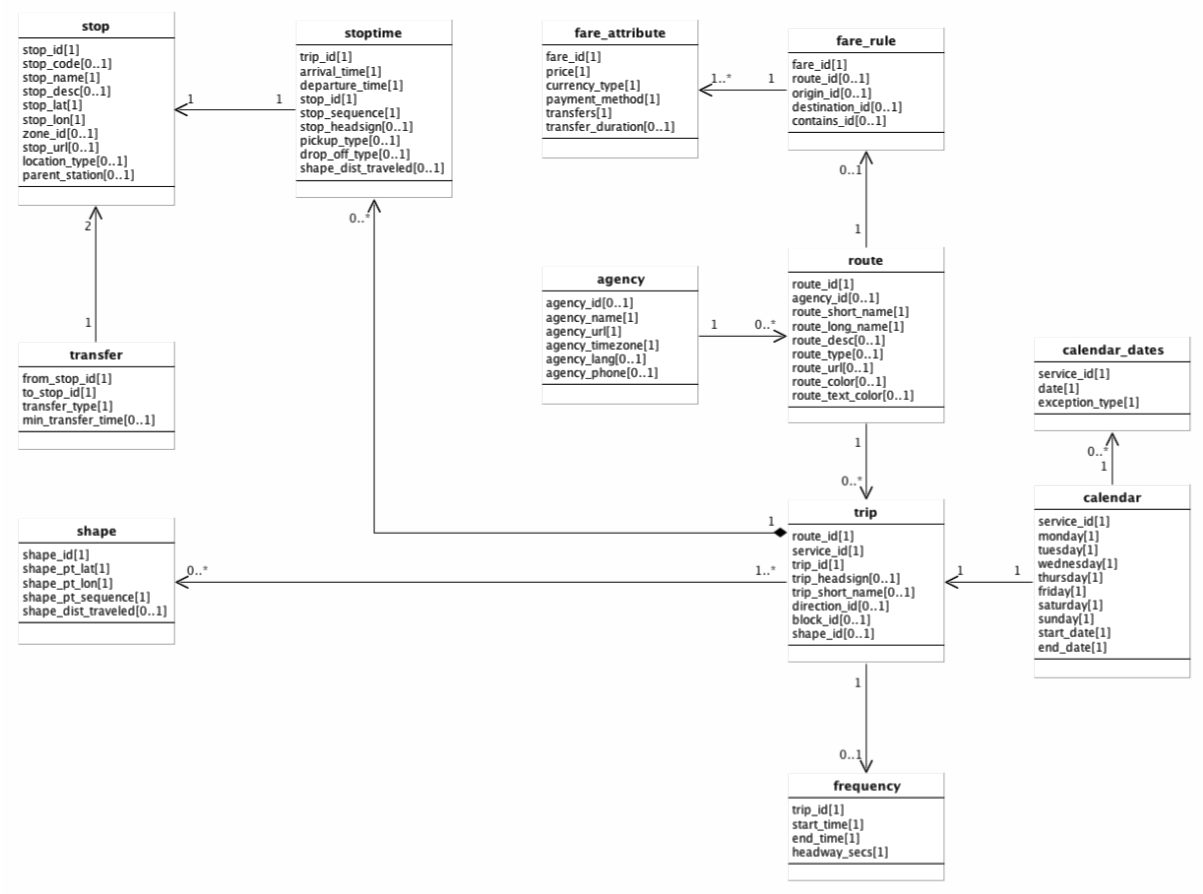
\includegraphics[scale=0.3]{kepek/gtfs_relationships.png}
\caption{A GTFS adatbázis tábláinak sémái és a közöttük lévő kapcsolatok.}
\label{fig:gtfs}
\end{figure}

A GTFS-formátum kötelező és opcionális táblákat egyaránt tartalmaz. A kötelező táblák létrehozása és adatokkal való feltöltése mindenképp szükséges a rendszer működéséhez.

\Section{Kötelező táblák}

\SubSection{agency}

A tömegközlekedési hálózat üzemeltetőjéről tartalmaz információkat. Több rekord is megadható, ha a járatokat több vállalat is üzemelteti. A route táblában minden viszonylatra meg lehet adni, hogy ki az üzemeltetője.

Kötelező mezők:

\begin{tabular}{|p{3cm}|p{10cm}|}
\hline
agency\_name & Az üzemeltető vállalt teljes neve. \\
\hline
agency\_url & A vállalat URL címe. \\
\hline
agency\_timezone & Az időzónát tartalmazza, ahol a vállalat található. \\
\hline
\end{tabular}

\SubSection{routes}

Az aktuálisan elérhető viszonylatokat tartalmazza. Minden viszonylat rendelkezik egy azonosítóval, egy rövid és egy hosszú névvel, valamint a viszonylat típusának az azonosítójával.
Kötelező mezők:

\begin{tabular}{|p{3cm}|p{10cm}|}
\hline
route\_id & Elsődleges kulcs, a viszonylat azonosítója. \\
\hline
route\_short\_name & A viszonylat rövid neve (száma). \\
\hline
route\_long\_name & A viszonylat hosszú neve, általában a két végállomást tartalmazza. \\
\hline
route\_type & Típusazonosító, lehetséges értékek:
0: villamos
1: metró
2: vasút
3: autóbusz
4: komp
5-7: egyéb járművek \\
\hline
\end{tabular}

\SubSection{trips}

Ez a tábla tartalmazza a járatokat. Mindegyik egy viszonylathoz tartozik, a direction\_id mezőben adható meg, hogy melyik irányban közlekedik a járat az adott viszonylaton (0 vagy 1 értékkel). Kötelező megadni még egy service\_id-t, ami alapján be lehet azonosítani, hogy a járat mely napokon közlekedik. Egy járathoz tartozhat még egy shape is, amely GPS koordináták sorozataként a járat útvonalát tartalmazza.
Kötelező mezők:

\begin{tabular}{|p{3cm}|p{10cm}|}
\hline
trip\_id & Elsődleges kulcs, a járat azonosítója. \\
\hline
route\_id & Idegen kulcs, a viszonylatra hivatkozik, amelyen a járat közlekedik. \\
\hline
service\_id & Idegen kulcs, a calendar és a calendar\_dates táblákra hivatkozik, ennek segítségével adható meg, hogy a járat mely napokon közlekedik. \\
\hline
\end{tabular}

\SubSection{stops}

Az egyes megállókat tárolja névvel és földrajzi koordinátákkal.
Kötelező mezők:

\begin{tabular}{|p{3cm}|p{10cm}|}
\hline
stop\_id & Elsődleges kulcs, a megálló azonosítója. \\
\hline
stop\_name & A megálló neve. \\
\hline
stop\_lat & A megálló szélességi fokát tartalmazza. A megadott értéknek WGS 84 szabvány szerintinek kell lenni. \\
\hline
stop\_lon & A megálló hosszúsági fokát tartalmazza. A megadott értéknek WGS 84 szabvány szerintinek kell lenni. \\
\hline
\end{tabular}

\SubSection{stop\_times}

Ez a tábla azt tárolja, hogy egy viszonylat egy járata egy megállóba mikor érkezik meg, mikor indul el onnan, és ez hányadik megállója az adott járatnak.
Kötelező mezők:

\begin{tabular}{|p{3cm}|p{10cm}|}
\hline
stop\_id & Idegen kulcs, a megálló azonosítója. \\
\hline
trip\_id & Idegen kulcs, a járat azonosítója. \\
\hline
arrival\_time & Érkezési idő, a járat mikor érkezik meg a megállóba. HH:MM:SS formátumban kell megadni. \\
\hline
departure\_time & Indulási idő, a járat mikor indul a megállóból. HH:MM:SS formátumban kell megadni. \\
\hline
stop\_sequence & Azt tartalmazza, hogy hányadik megállója ez a járatnak. Nemnegatív egésznek kell lennie. \\
\hline
\end{tabular}

\SubSection{calendar}

Itt úgynevezett szolgáltatásokat lehet megadni. Egy szolgáltatás azt mondja meg, hogy a járatok, amelyek ehhez a szolgáltatáshoz tartoznak, a hét mely napjain közlekednek. Továbbá meg kell adni egy érvényességi intervallumot is.
Kötelező mezők:

\begin{tabular}{|p{3cm}|p{10cm}|}
\hline
service\_id & Elsődleges kulcs, a szolgáltatás azonosítója. \\
\hline
Monday & Azt mondja meg, hogy az adott napon közlekedik-e a járat.
Az értéke lehet:
0, ha az adott napon nem közlekedik, és
1, ha az adott napon közlekedik a járat.
Tuesday

Wednesday

Thursday

Friday

Saturday

Sunday\\
\hline
start\_date & A szolgáltatás kezdő érvényességi ideje. Az értéket YYYYMMDD formátumban kell megadni. \\
\hline
end\_date & A szolgáltatás érvényességi idejének a vége. Az értéket YYYYMMDD formátumban kell megadni. \\
\hline
\end{tabular}

Opcionális táblák:

\SubSection{shapes}

A járatok útvonalát tartalmazza a tábla. Egy útvonal több pontból áll, amelyek ugyanazzal a shape\_id-val vannak ellátva.
Kötelező mezők:

\begin{tabular}{|p{3cm}|p{10cm}|}
\hline
shape\_id & Az útvonal azonosítója. \\
\hline
shape\_pt\_lat & Az útvonal egy pontjának szélességi fokát tartalmazza. A megadott értéknek WGS 84 szabvány szerintinek kell lenni. \\
\hline
shape\_pt\_lon & Az útvonal egy pontjának hosszúsági fokát tartalmazza. A megadott értéknek WGS 84 szabvány szerintinek kell lenni. \\
\hline
shape\_pt\_sequence & Azt tartalmazza, hogy hányadik pontja ez a útvonalnak. Nemnegatív egésznek kell lennie. \\
\hline
\end{tabular}

\SubSection{calendar\_dates}

A táblának két felhasználási módja van.
Ajánlott: A calendar táblával együttesen, ilyenkor a normál menetrend szerinti kivételes eseteket kell itt megadni.
Alternatív: A calendar táblát kihagyva, csak ezt a táblát használni, az összes szolgáltatást itt megadva. 
Kötelező mezők:

\begin{tabular}{|p{3cm}|p{10cm}|}
\hline
service\_id & A szolgáltatás azonosítója. Egy (service\_id, date) páros csak egyszer szerepelhet. \\
\hline
date & Egy dátumot tartalmaz, formátuma: YYYYMMDD. \\
\hline
exception\_type & Lehetséges értékei:
1, ha a szolgáltatást hozzá akarjuk adni az adott naphoz, és
2, ha a szolgáltatást el szeretnék távolítani a megadott napon. Például: ha egy járat közlekedik hétfőnként, de egy ünnep hétfőre esik, így tudjuk megadni, hogy aznap a járat nem közlekedik. \\
\hline
\end{tabular}

\SubSection{fare\_attributes}

A különböző viteldíjtípusok megadására szolgál.
Kötelező mezők:

\begin{tabular}{|p{3cm}|p{10cm}|}
\hline
fare\_id & A viteldíj azonosítója. \\
\hline
price & A viteldíj ára a currency\_type mezőben meghatározott egységben kifejezve. \\
\hline
currency\_type & A valuta ISO 4217 szabvány szerinti kódja. \\
\hline
payment\_method & Azt határozza meg, hogy a viteldíjat mikor kell kifizetni.
Lehetséges értékei:
0, ha felszálláskor kell fizetni, és
1, ha felszállás előtt kell fizetni. \\
\hline
transfers & Azt specifikálja, hogy hány átszállás lehetséges az adott viteldíjtípussal.
Lehetséges értékei:
0: nem engedélyezett az átszállás
1: egy átszállás engedélyezett
2: két átszállás engedélyezett
üres: ha a mező üres, akkor bármennyi átszállás engedélyezett. \\
\hline
\end{tabular}

\SubSection{fare\_rules}

A táblával megadható, hogy a fare\_attributes táblában található viteldíjak hogyan vonatkozzanak az útvonalakra.
Kötelező mező:

\begin{tabular}{|p{3cm}|p{10cm}|}
\hline
fare\_id & Idegen kulcs, a viteldíjat azonosítja. \\
\hline
\end{tabular}

Opcionális mezők:

\begin{tabular}{|p{3cm}|p{10cm}|}
\hline
route\_id & Idegen kulcs, a viszonylat azonosítója. Ha több viszonylathoz is ugyanaz a viteldíj tartozik, akkor minden egyes viszonylatot külön rekordként kell felvinni a táblában. \\
\hline
origin\_id & Idegen kulcsok, a stops tábla zone\_id mezőire hivatkozhatnak. \\
\hline
destination\_id &  \\
\hline
contains\_id & \\
\hline
\end{tabular}

\SubSection{frequencies}

Ha egy járat szerepel ebben a táblában, akkor az útvonaltervező figyelmen kívül hagyja a stop\_times tábla arrival\_time és departure\_time mezőjét. Ehelyett a stop\_times tábla a megállók sorrendjét és az egyes megállók közötti időkülönbséget határozza meg.
Kötelező mezők:

\begin{tabular}{|p{3cm}|p{10cm}|}
\hline
trip\_id & Idegen kulcs, egy járatra hivatkozik. \\
\hline
start\_time & Az az időpont, amikor az első jármű elhagyja a járat első megállóját. \\
\hline
end\_time & Az az időpont, amikor a járat egy másik gyakoriságra vált. \\
\hline
headway\_secs & Másodpercekben kifejezve, hogy a start\_time és az end\_time mezők által meghatározott időintervallumon belül mennyi idő telik el két indulás között ugyanabból a megállóból. \\
\hline
\end{tabular}

\SubSection{transfers}

Útvonaltervezők általában az átszállási pontokat az egyes viszonylatok megállóinak a távolságai alapján számítják ki. Az esetlegesen kétértelmű megálló párok egyértelműsítésére vagy egy konkrét csatlakozási lehetőség megadására szolgál ez a tábla.
Kötelező mezők:

\begin{tabular}{|p{3cm}|p{10cm}|}
\hline
from\_stop\_id & Idegen kulcs. Egy megálló azonosítóját tartalmazza, ahol a viszonylatok közti kapcsolat kezdődik.  \\
\hline
to\_stop\_id & Idegen kulcs. Egy megálló azonosítóját tartalmazza, ahol a viszonylatok közti kapcsolat végződik. \\
\hline
transfer\_type & A két megálló (from\_stop\_id, to\_stop\_id) közti kapcsolat típusát adja meg.
Lehetséges értékek:
0 vagy üres: Ajánlott átszállási pont a viszonylatok között.
1: Időzített átszállási pont két viszonylat között. Az induló jármű megvárja az érkezőt, elegendő időt biztosítva az utasok számára az átszálláshoz.
2: Az átszállás biztosításához bizonyos idő szükséges. Az ehhez szükséges időt a min\_transfer\_time mező tartalmazza.
3: Az adott helyen átszállás nem lehetséges a viszonylatok között. \\
\hline
\end{tabular}

\SubSection{feed\_info}

Ez a tábla az adatokat publikáló szervezetről tartalmaz információkat. Abban az esetben van fontosabb szerepe, ha a tömegközlekedési hálózat üzemeltetője és az adatok publikálója nem ugyanaz a szervezet.
Kötelező mezők:

\begin{tabular}{|p{3cm}|p{10cm}|}
\hline
feed\_publisher\_name & Az adatokat szolgáltató szervezet teljes neve. Általában megegyezik az agency tábla agency\_name mezőével. \\
\hline\
feed\_publisher\_url & Az adatokat szolgáltató szervezet URL címe. Általában megegyzik az agency tábla agency\_url mezőével. \\
\hline
feed\_lang & A szövegek alapértelmezett nyelvének IETF BCP 47 nyelvkódját tartalmazza. \\
\hline
\end{tabular}

\Section{GTFSDB}

A nyers GTFS-adatok feldolgozásához először a Google TransitFeed modulját kezdtem el használni. Ennek segítségével a memóriába be tudtam tölteni az adatokat, amiknek a lekérdezésére és a módosítására is lehetőség volt. Azonban hamar arra a következtetésre jutottam, hogy ez számomra nem lesz tökéletesen megfelelő, hiszen én mindenféleképpen adatbázisban szeretném tárolni az adatokat. A Google által kifejlesztett API segítségével is lehet az adatokat lekérdezni és módosítani, azonban úgy gondoltam, hogy az adatbázisban történő tárolással több és jobb lehetőség nyílik erre. A másik ok, amiért erre a következtetésre jutottam, hogy az adatokat ezáltal perzisztensen tudom tárolni.

Elkezdtem ilyen megoldás után kutakodni, így találtam rá az OpenTransitTools GTFSDB nevű könyvtárára. A projekt célja, hogy a GTFS-adatokat programozható kontextusba helyezze szoftverfejlesztők számára. Ennek igen nagy létjogosultsága van, hiszen a GTFS-adatokkal foglalkozó alkalmazások készítésénél általában az első lépés a nyers adatok lekérdezhetővé, feldolgozhatóvá tétele. A GTFSDB könyvtár segítségével PostgreSQL, Oracle, MySQL és SQLite adatbázisokat hozhatunk létre a nyers adatokból. A projekt forráskódja elérhető GitHubon: https://github.com/OpenTransitTools/gtfsdb

\begin{python}
path = resource_filename('gtfsdb', 'zips')
gtfs_file = 'file:///{0}'.format(os.path.join(path, 'mvkzrt.zip'))
basedir = os.path.abspath(os.path.dirname(__file__))
url = 'sqlite:///' + os.path.join(basedir, 'mvk.db')
db = database_load(gtfs_file, url=url)
\end{python}

Az adatbázis létrehozása és feltöltése a database\_load függvény meghívásával történik. Paraméterként meg kell adni a GTFS-adatokat tartalmazó .zip fájlt, illetve a létrehozni kívánt adatbázisfájl helyét, nevét és típusát. Ezt lefuttatva létrejönnek a táblák és feltöltődnek adatokkal. Ez után már SQLAlchemy segítségével könnyedén lekérdezhetővé válnak az adatok.

A GTFSDB-t Python 2.7-es verzióval ajánlott használni, így először én is azzal próbáltam. Ezáltal viszont a következő problémába ütköztem bele. Az adatbázis feltöltése közben hiba keletkezett, nem sikerült az ékezetet tartalmazó szövegek feldolgozása. Témavezetőm azt tanácsolta, hogy próbáljam meg a Python 3-as verziójával lefuttatni a kódot, és akkor valószínűleg az ékezetes betűkből adódó karakterkódolási hiba meg fog szűnni. Ahhoz, hogy a GTDSDB működjön Python 3-mal, ahhoz a forráskódjában néhány sort át kellett írni. A következőkben ezeket a változtatásokat ismertetem.

gtfsdb/config.py

1. sor:
\begin{python}
-from ConfigParser import ConfigParser
+from configparser import ConfigParser
\end{python}

gtfsdb/model/base.py

33. sor:
\begin{python}
-except Exception, e:
+except Exception as e: 
\end{python}

158. sor:
\begin{python}
-if isinstance(v, basestring):
+if isinstance(v, str):
\end{python}

171. sor:
\begin{python}
-except Exception, e:
+except Exception as e:
\end{python}

gtfsdb/model/db.py

82. sor:
\begin{python}
-except Exception, e:
+except Exception as e:
\end{python}

gtfsdb/model/gtfs.py

6. sor:
\begin{python}
-from urllib import urlretrieve
+from urllib.request import urlretrieve
\end{python}

53. sor:
\begin{python}
-except Exception, e:
+except Exception as e:
\end{python}

gtfsdb/model/route\_stop.py

260. sor:
\begin{python}
-print unique_stops
+print(unique_stops)
\end{python}

gtfsdb/model/stop\_time.py

75. sor:
\begin{python}
-except Exception, e:
+except Exception as e:
\end{python}

Ezekkel a változtatásokkal, Python 3 alatt, sikeresen lefutott a database\_load függvény ékezetes karaktereket tartalmazó forrásfájlok esetén is.


\Chapter{A szerveroldali rész megvalósítása}

Szerveroldalon egy többrétegű struktúrát alakítottam ki, mint azt már említettem az alkalmazás felépítésének a részletezésénél. A fejezetben a két felső réteg, a Flask-alkalmazás és a menetrend csomag kerül bemutatásra.

\Section{Flask-webalkalmazás}

% Azt kellene bemutatni, hogy az menetrend lib funkcióit hogy sikerült kivezetni, hogy REST API-n keresztül elérhető legyen.
Ez a réteg dolgozza fel a klienstől érkező kéréseket a menetrend csomagra építve. Ha vannak a kérésnek paraméterei, akkor először azoknak a helyességét vizsgálja. Számos esetben ezt egy, a menetrend csomagban lévő, függvény segítségével végzi. A válaszokhoz az adatokat szintén a menetrend csomag egyes függvényeinek a meghívásával állítja elő. Az így előállt eredményadatokat JSON formátumban küldi a kliens felé.
A réteg a server.py fájlban van megvalósítva. A benne található függvények route() dekorátorokkal vannak ellátva. Ezek írják le, hogy mely URL-re hívódjon meg az adott függvény. Az URL-ek és a függvények nevei az egyszerűség kedvéért megegyeznek.
A függvényeket és leírásukat tartalmazza a következő táblázat.

\begin{longtable}{|p{4.5cm}|p{9cm}|}
\hline
\textbf{URL} & \textbf{Leírás} \\
\hline
\texttt{/} &
Az alkalmazás megnyitásakor vagy a főoldal gombra történő kattintáskor elküldi az index.html fájlt. \\
\hline
\texttt{/favicon.ico} &
A favicon megjelenítésére szolgál. A favicon a weboldalhoz tartozó ikon, amely a böngészőben megjelenhet a címsorban, a fül elején és a könyvjelzők előtt. \\
\hline
\texttt{/get\_bus\_routes} &
Az autóbuszvonalakat adja vissza. A lekérdezéshez a \texttt{query\_routes\_by\_route\_type()} függvényt hívja meg. A paraméter adja meg a típust, a 3-as jelenti az autóbuszt. \\
\hline
\texttt{/get\_tram\_routes} &
A villamosvonalakat adja vissza. A fent említett függvényt hívja meg, 0-t adva paraméterként, hiszen ez jelenti a villamostípust. \\
\hline
\texttt{/get\_start\_times} &
Egy viszonylat egy irányának egy adott napi indulási idejeit adja vissza.
Paraméterek:
\begin{itemize}
\item \texttt{route\_short\_name}: a viszonylatot határozza meg
\item \texttt{direction\_id}: az irányt határozza meg
\item \texttt{date}: a dátumot határozza meg
\end{itemize}
A függvény először a paraméterek helyességét vizsgálja. Ha a \texttt{direction\_id} értéke nem 0 vagy 1, vagy ha egy járat sem található a megadott \texttt{route\_short\_name} és \texttt{direction\_id} értékekkel, akkor 404-es hibakóddal tér vissza. Ennek az az oka, hogy ez normál használat során nem fordulhat elő, csak ha kézzel át lett írva az URL.
Ha helyesek a paraméterek, akkor a \texttt{query\_trips\_schedule()} függvény segítségével lekérdezi a paramétereknek megfelelő járatokat. Ha egyet sem talál, akkor az adott napon nem közlekedik a viszonylat. Ellenkező esetben a \texttt{generate\_schedule\_dictionary()}  függvénnyel elkészíti az aznapi indulási időket tartalmazó dictionary-t. \\
\hline
\texttt{/get\_dates} &
Az adatbázisban a menetrendi adatokhoz tartozó dátumokat adja vissza. Ezekből a dátumokból lehet választani a menetrendböngésző oldalon. A lekérdezéshez a \texttt{query\_dates()} függvényt használja.  \\
\hline
\texttt{/get\_trip\_stops} &
Egy járat részletes menetrendjét adja vissza. Paraméterként egy \texttt{trip\_id}-t kap, először teszteli, hogy valós-e. Ha nem, 400-as hibakóddal tér vissza. Ha igen, akkor a \texttt{query\_trip\_stops()} függvénnyel lekérdezi a járat menetrendjét.  \\
\hline
\texttt{/get\_trip\_shapes} &
Egy járat útvonalát adja vissza. Paraméterként egy \texttt{trip\_id}-t kap, először teszteli, hogy valós-e. Ha nem, 400-as hibakóddal tér vissza. Ha igen, akkor a \texttt{query\_trip\_shapes()} függvénnyel lekérdezi a járat útvonalát. \\
\hline
\texttt{/get\_trip\_terminals} \\ \texttt{\_coordinates} &
Egy járat induló és végállomásának a koordinátáit adja vissza. Paraméterként egy \texttt{trip\_id}-t kap, először teszteli, hogy valós-e. Ha nem, 400-as hibakóddal tér vissza. Ha igen, akkor a \texttt{query\_trip\_terminals\_coordinates()} függvénnyel lekérdezi az említett koordinátákat. \\
\hline
\texttt{/get\_trip\_stops\_} \\ \texttt{coordinates} &
Egy járat megállóinak a koordinátáit adja vissza, kivéve az indulóét és a végállomásét. Paraméterként egy \texttt{trip\_id}-t kap, először teszteli, hogy valós-e. Ha nem, 400-as hibakóddal tér vissza. Ha igen, akkor a \texttt{query\_trip\_stops\_coordinates()} függvénnyel lekérdezi az említett koordinátákat. \\
\hline
\texttt{/get\_all\_stops} &
Az adatbázisban található összes megálló nevét adja vissza. A lekérdezéshez a \texttt{query\_all\_stops()} függvényt használja. \\
\hline
\texttt{/plan\_trip} &
A megadott induló és célmegálló közt tervezett útvonalat adja vissza. Az útvonaltervezéshez a \texttt{dijkstra()} függvényt használja. \\
\hline
\end{longtable}

\Section{A menetrend library}

A csomagban található függvényekkel lehet az adatbázisból adatok lekérdezni, az SQLAlchemy és a GTFSDB segítségével. A következő táblázat a csomagban lévő fájlokat és az azokban lévő függvényeket ismerteti.

\begin{longtable}{|p{4.5cm}|p{9cm}|}
\hline
\textbf{Fájlnév} & \textbf{Függvények leírásai} \\
\hline
\texttt{graph.py} &
\texttt{generate\_graph()}:

Az adatbázisban található megállókból egy súlyozott, irányított gráfot épít fel, az alapján, hogy honnan hova és mennyi idő alatt lehet eljutni. A függvény működése a hetedik fejezetben részletesen ki van fejtve.
\\
\hline
\texttt{routes.py} &
\texttt{query\_routes\_by\_route\_type(route\_type)}:

Az adatbázisból a paraméterként megadott típusú viszonylatokat kérdezi le, dictionary-k listájaként visszaadva az eredményt.

\bigskip

\texttt{test\_route\_short\_name(route\_short\_name, direction\_id)}:

Megvizsgálja, hogy a paraméterként megadott viszonylatnév létezik-e az adatbázisban. Ha igen, akkor visszatér vele.
\\
\hline
\texttt{schedule.py} &
\texttt{query\_dates()}:

Az adatbázisban a menetrendi adatokhoz tartozó dátumokat adja vissza egy listában.

\bigskip

\texttt{query\_trips\_schedule(route\_short\_name, direction\_id, date, trip)}:

A paramétereknek megfelelő járatokat és a járatok adatait tartalmazó dictionary-t adja vissza.

\bigskip

\texttt{generate\_schedule\_dictionary(trips, trips\_dict)}:

A paraméterként kapott járatok indulási időivel kibővíti a paraméterként átadott dictionary-t, majd ezzel a kibővített dictionary-vel tér vissza.
\\
\hline
\texttt{stops.py} &
\texttt{query\_all\_stops()}:

Az adatbázisban található összes megálló nevét adja vissza egy listában.
\\
\hline
\texttt{trip\_planner.py} &
\texttt{dijkstra(graph, src, dest)}:

Dijkstra-algoritmus a gráfban való legrövidebb út megkeresésére két megálló között. Az algoritmus a hetedik fejezetben kerül részletes bemutatásra.
\\
\hline
\texttt{trips.py} &
\texttt{test\_trip(trip\_id)}:

Megvizsgálja, hogy a paraméterként kapott azonosítójú járat létezik-e az adatbázisban. Ha létezik, visszatér vele.

\bigskip

\texttt{query\_trip\_stops(trip):}

Egy dictionary-ben visszaadja a paraméterként kapott járat nevét, induló és végállomását, valamint a dictionary-n belül egy listában a sorrendben érintett megállókat, indulási idővel és az adott megállóig eltelt menetidővel.

\bigskip

\texttt{query\_trip\_shapes(trip)}:

A paraméterként megadott járat útvonalát adja vissza egy listában.

\bigskip

\texttt{query\_trip\_terminals\_coordinates(trip)}:

A paraméterként megadott járat induló és végállomásának a koordinátáit adja vissza egy listában.

\bigskip

\texttt{query\_trip\_stops\_coordinates(trip)}:

Egy listában a paraméterként megadott járat megállóinak a koordinátáit adja vissza, kivéve az indulóét és a végállomásét.
\\
\hline
\end{longtable}

A menetrend csomagnak számos előnye van véleményem szerint. Egyrészt ennek a rétegnek a bevezetésével jobban el tudtam különíteni az egyes funkciókat. A flaskos réteg csak a kérések helyességének vizsgálatával és a válaszok generálásával foglalkozik. A lekérdezések megfogalmazása és az eredmények feldolgozása a menetrend csomag függvényeiben történik, ezáltal átláthatóbb is lett a Flask-fájl, hiszen rövidebbek az egyes függvények törzsei.

A legnagyobb előny, véleményem szerint, a jövőbeli továbbfejleszthetőség nagymértékű megkönnyítésében rejlik. Ha később úgy döntök (vagy bárki más úgy dönt), hogy a MEnetrend webalkalmazásnak el kívánom (kívánja) készíteni a mobilos vagy asztali változatát, akkor a back enden csak a Flaskot kell lecserélni, az alsóbb rétegekben megvalósított funkciók ugyanazok maradhatnak. Esetleg egy másik, hasonló tematikájú webalkalmazás is építkezhet a menetrend csomagban megvalósított néhány funkcióra.

% A menetrend library, mint wrapper a GTFSDB felé

% Az előnye, hogy így más kliensekkel is lehet használni (mobil, desktop app, vagy másik webapp).

\Chapter{A front end megvalósítása}

% TODO: Minden képet be kell majd hivatkozni!

% TODO: A szövegben ki kell emelni a kódrészeket texttt{}-vel! ..vagy textit-vel, csak következetes legyen!

\Section{Felhasználói felület elemei}

Az alkalmazás főoldalán egy ismertető található, a program funkcionalitását bemutatva.
A felhasználói felületének két fő része van, a menetrendadatok böngészése és az útvonaltervezés. Ezeket a navigációs sávon külön menüpontokból érhetjük el.

\begin{figure}[h!]
\centering
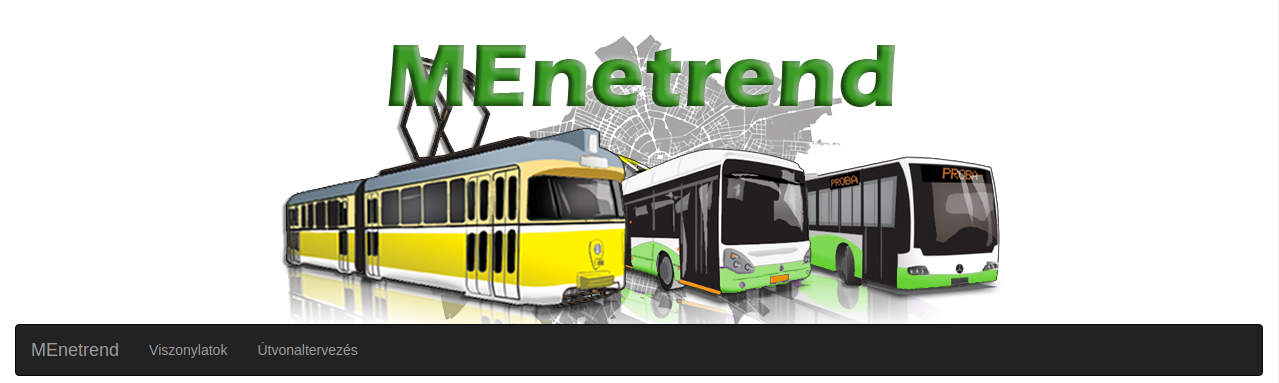
\includegraphics[scale=0.32]{kepek/navbar.png}
\caption{Az alkalmazás navigációs sávja}
\label{fig:navbar}
\end{figure}

A navigációs sávon (\ref{fig:navbar}. ábra) a Viszonylatok menüpontra kattintva láthatjuk a különböző viszonylatokat, ahol többféle módon is kiválaszthatjuk azt, amelyiknek a menetrendjére kíváncsiak vagyunk. Található az oldal tetején egy gombsor a vonalszámokkal (\ref{fig:viszonylatok_gombsor}. ábra), alatta pedig egy részletes táblázat, csoportosítva a különböző típusú viszonylatokat.

\begin{figure}[h!]
\centering
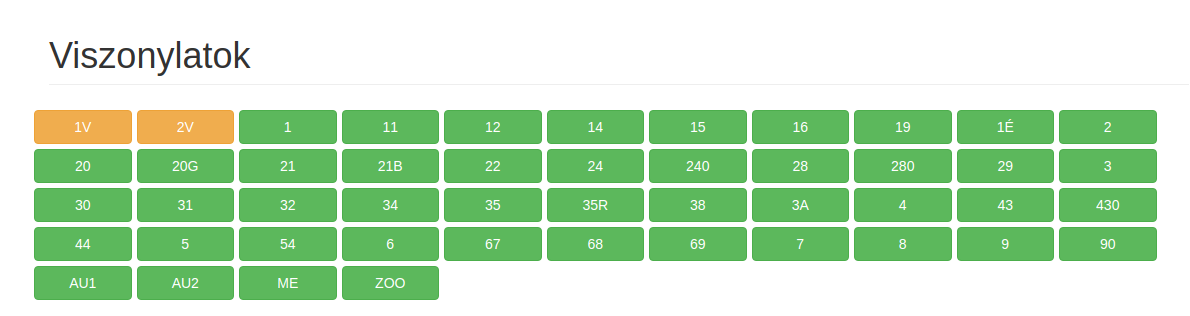
\includegraphics[scale=0.32]{kepek/viszonylatok_gombsor.png}
\caption{Gombsor a vonalszámokkal}
\label{fig:viszonylatok_gombsor}
\end{figure}

\Aref{fig:vonalak_tablazat}. ábrán látható táblázat három oszlopból áll: vonalszám, induló állomás és érkező állomás. Lehetőség van bármelyik oszlop szerint csökkenő vagy növekvő sorrendben rendezni a táblázatot vagy keresni benne. A Keresés mezőbe beírt szöveg alapján a táblázat mindegyik oszlopában keres egyezőséget, a szűrés az oldal újratöltése nélkül megtörténik. A keresés kis- és nagybetű-érzéketlen.

\begin{figure}[h!]
\centering
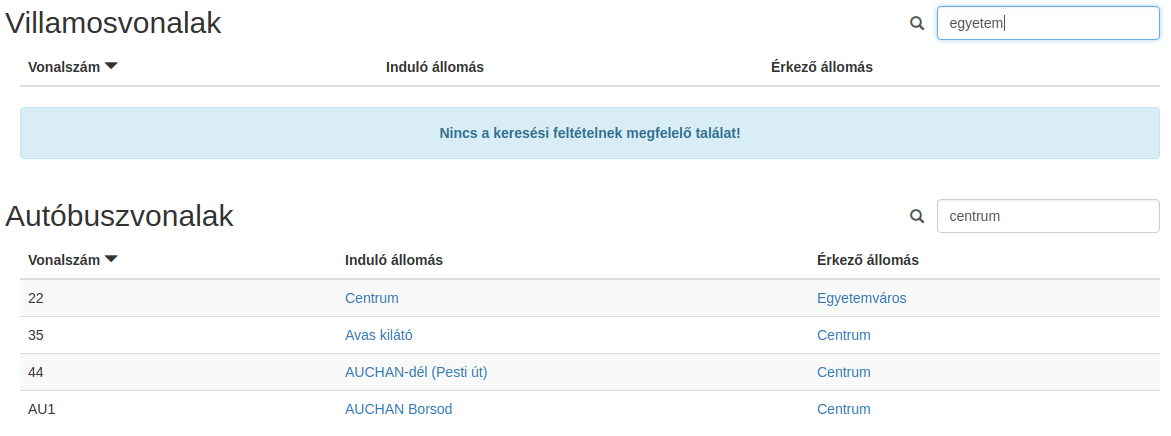
\includegraphics[scale=0.32]{kepek/vonalak_tablazat.png}
\caption{A vonalszámokat, indulóállomásokat és az érkező állomásokat megjelenítő táblázat}
\label{fig:vonalak_tablazat}
\end{figure}

Ha kiválasztunk egy viszonylatot, akkor annak az aznapi menetrendjét látjuk egy óra-perc táblázatban (\ref{fig:menetrend}. ábra). A táblázat mellett egy legördülő menüből lehet a napot választani, ha a vonal egy másik napi menetrendjére vagyunk kíváncsiak.

\begin{figure}[h!]
\centering
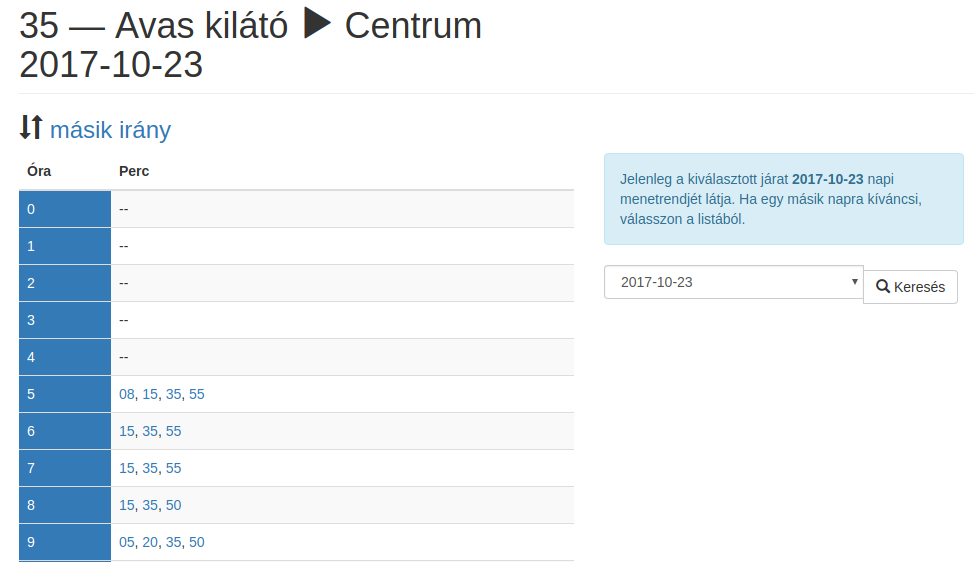
\includegraphics[scale=0.4]{kepek/menetrend.png}
\caption{Az adott nap menetrendje óra-perc táblázatos formában}
\label{fig:menetrend}
\end{figure}

A táblázatban a percek linkek, amire ha rákattintunk, akkor egy másik oldal töltődik be, amit \aref{fig:trip_tablazat_es_terkep}. ábrán láthatunk. Ez az oldal is két részre van felosztva. Bal oldalt egy táblázatban láthatjuk a kiválasztott járat részletes menetrendjét, sorrendben az állomásokat, amiket érint. Három oszlopból áll a táblázat: indulási idő, megálló neve, és az addigi menetidő percben kifejezve. A táblázat mellett pedig a járat útvonala jelenik meg Google Mapsen. A térképen a járat útvonala és az érintett megállók is fel vannak tüntetve. A megállókat jelző \texttt{markerekre} kattintva egy \texttt{InfoWindow} ugrik fel, a megálló nevét és a járat végállomását tartalmazva.

\begin{figure}[h!]
\centering
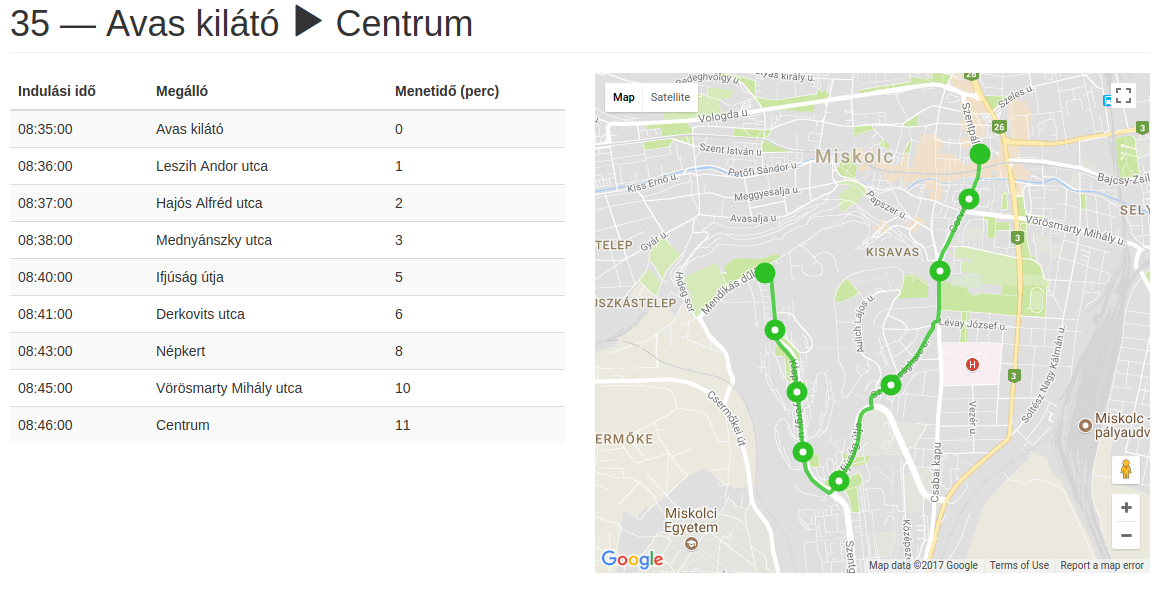
\includegraphics[scale=0.35]{kepek/trip_tablazat_es_terkep.png}
\caption{Egy járat megállóinak és útvonalának megjelenítése táblázatos és térképes formában}
\label{fig:trip_tablazat_es_terkep}
\end{figure}

Az alkalmazás másik fő funkcióját is a navigációs sávról érhetjük el, ez nem más, mint az útvonaltervezés. Az oldal két részre van felosztva, ahogy \aref{fig:trip_planner}. ábrán látható.

Bal oldalt az útvonaltervezés beállításait adhatjuk meg. Az első sorban a kezdő- és a célmegállót állíthatjuk be két input mező segítségével, amit \textit{autocomplete} támogatás is segít. Ez azt jelenti, hogy ha elkezdünk gépelni a beviteli mezőbe, akkor megjelenik egy legördülő listához hasonlító elem, amiből kiválaszthatjuk a megfelelő megálló nevét. \Aref{fig:autocomplete}. ábrán megfigyelhető, hogy ez mit is jelent a gyakorlatban. A második sorban a Tervezés gomb található.

Jobb oldalt, miután a Tervezés gombra kattintottunk, a kérés eredménye látható. Ha megfelelő adatokat adtunk meg, és létezik útvonal a két megálló közt, akkor megjelenik a javasolt útvonal. Ellenkező esetben egy hibaüzenet jelenik meg.

\begin{figure}[h!]
\centering
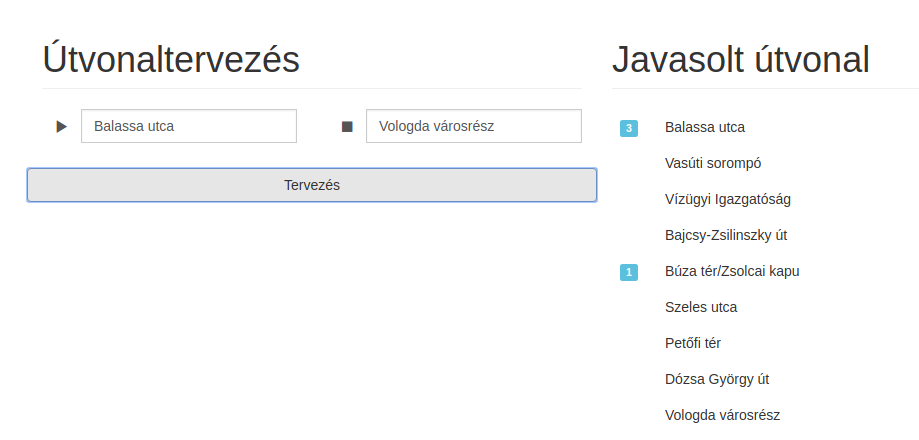
\includegraphics[scale=0.45]{kepek/trip_planner.png}
\caption{Útvonaltervezés}
\label{fig:trip_planner}
\end{figure}

\begin{figure}[h!]
\centering
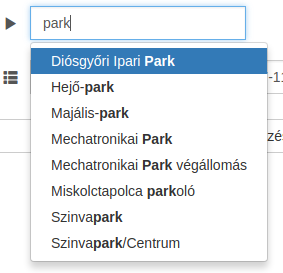
\includegraphics[scale=0.6]{kepek/autocomplete.png}
\caption{Automatikus kiegészítés a keresés segítéséhez}
\label{fig:autocomplete}
\end{figure}

\Section{Megvalósítás AngularJS segítségével}

A bemutatott felületek kialakítása AngularJS-sel történt. Az AngularJS kontrollerei kommunikálnak a szerverrel, az adatok nézeteken való megjelenítését biztosítják. Ezt az \texttt{app.js} fájl valósítja meg.
Az alkalmazás single-page application, ami azt jelenti, hogy egy oldal tartalma változik dinamikusan az alkalmazás használata során, nem teljesen különböző oldalak töltődnek le a szerverről. Különböző állapotok vannak definiálva, amiket a \texttt{\$stateProvider} modul kezel. Egy állapot definiálása a \texttt{\$stateProvider .state()} metódusával történik.
Egy állapot definiálása a következőképpen történik:
\begin{cpp}
.state("/trip", {
            url: "/trip/{trip_id:int}",
            templateUrl: "/static/partials/trip.html",
            controller: "tripController"
        })
\end{cpp}
Meg kell adni az állapot nevét, milyen URL-re aktiválódjon, melyik nézetet töltse be és melyik kontrollert használja hozzá.
Az \texttt{\$urlRouterProvider} segítségével létrehoztam egy úgynevezett \textit{otherwise} állapotot, ami akkor aktiválódik, ha az adott URL egyik állapot URL-ére sem illeszkedik. Ilyenkor egy erre figyelmeztető hibaüzenetet tartalmazó nézet töltődik be. Ezt mutatja \aref{fig:404}. ábra.

\begin{figure}[h!]
\centering
\frame{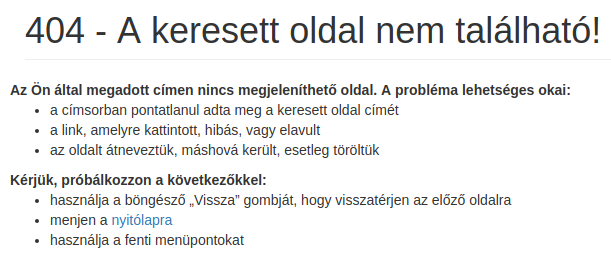
\includegraphics[scale=0.7]{kepek/404.png}}
\caption{404-es hibajelzés abban az esetben, ha a lap nem található}
\label{fig:404}
\end{figure}

A nézetek \texttt{.html} fájlokban vannak tárolva, ezek azonban nem teljes \texttt{.html} fájlok, csupán HTML-kódrészletek. Minden nézethez definiáltam egy kontrollert is, ezáltal jól elkülönítve az egyes állapotok kódjait.

Az elkészített nézetek és kontrollerek összefoglalása látható \aref{tab:routing}. táblázatban.

\begin{figure}[h!]
\centering
\begin{tabular}{|l|p{4cm}|l|}
\hline
\textbf{Nézet, \texttt{/static/partials/}} & \textbf{URL} & \textbf{Kontroller neve} \\
\hline
\texttt{home.html} & \texttt{/} & \texttt{-} \\
\hline
\texttt{list-routes.html} & \texttt{/list-routes} & \texttt{listRoutesController} \\
\hline
\texttt{trip.html} & \texttt{/trip/{trip\_id:int}} & \texttt{tripController} \\
\hline
\texttt{schedule.html} &
\texttt{/schedule/}

\texttt{:route\_short\_name/}

\texttt{\{direction\_id:int\}} & \texttt{scheduleController} \\
\hline
\texttt{trip-planner.html} & \texttt{/trip-planner} & \texttt{tripPlannerController} \\
\hline
\texttt{error-404.html} & \texttt{/error-404} & \texttt{-} \\
\hline
\end{tabular}
\caption{Routing: nézet, url, controller}
\label{tab:routing}
\end{figure}

A \texttt{listRoutesController} a viszonylatokat kéri le a szervertől a viszonylatok típusa szerint csoportosítva. A megjelenített táblázatokban a különböző oszlopok szerinti rendezést és a bennük való keresést valósítja meg.
A \texttt{tripController} egy járat adatait kéri le a szervetől. Amennyiben hibás paramétert kap, a 404-es hibaoldalra irányít át.
A \texttt{scheduleController} az adatbázisban található dátumokat és egy viszonylat napi indulási adatait kéri le a szervertől. Alapértelmezetten az aktuális dátum szerinti menetrendet kérdezi le. Ha a nézeten a napválasztó legördülő menüből egy másik napot választ ki a felhasználó, akkor a kiválasztott nap menetrendjét kérdezi le.
A \texttt{tripPlannerController} lekérdezi az adatbázisban található megállók neveit, és a dátumokat. A hozzátartozó nézeten található formon bevitt adatokat validálja, ha hibásak, akkor megjeleníti a hibaüzenetet a nézeten. Ha a megadott adatok megfelelőek, elküldi azokat a szervernek, a válaszként kapott megtervezett útvonalat pedig megjeleníti a nézeten. Ha nem talált útvonalat az algoritmus, akkor szintén egy hibaüzenetet jelenít meg.

\Section{Térképadatok kezelése és megjelenítése}

A járatok útvonalának térképen történő megjelenítésére a Google Mapset használtam. Döntésemet az indokolta, hogy véleményem szerint a piacon jelenlévő térképszolgáltatások közül messze a Google-é a legfejlettebb, legtámogatottabb. A térkép programozására a Google Maps JavaScript API-t használtam. Ennek segítségével JavaScriptben írt kóddal tudjuk programozni a térképet. Számos funkciót kínál erre az API, én legfőképp az útvonalak kirajzolását és jelölőpontok megjelenítését használtam. Ahhoz, hogy oldalunkon használni tudjuk az API-t, be kell szereznünk egy úgynevezett API key-t. Ezt a következő oldalon tudjuk megtenni: \url{https://code.google.com/apis/console}.

Az oldalon létre kell hozni egy projektet, majd ki kell választani, hogy melyik API-ra van szükségünk. Én a Google Maps JavaScript API-t választottam ki, ezután meg is kaptam a szükséges kulcsot. Lehetőség van arra is, hogy lekorlátozzuk a kulcs használatát. Megadhatjuk, hogy mely domain címekről használhatják a kulcsunkat. Ingyenesen napi 25 000 darab kérésünk lehet, ami egy átlagos forgalmú weboldal esetén elegendő. Ha azonban mégis átlépné az oldalunk ezt a napi limitet, akkor vásárolhatunk üzleti csomagot, amivel lehetőségünk van kibővíteni ezt a keretet. \Aref{fig:google_maps_api_1}. ábrán látható az adminisztrációs felületről egy kép.

\begin{figure}[h!]
\centering
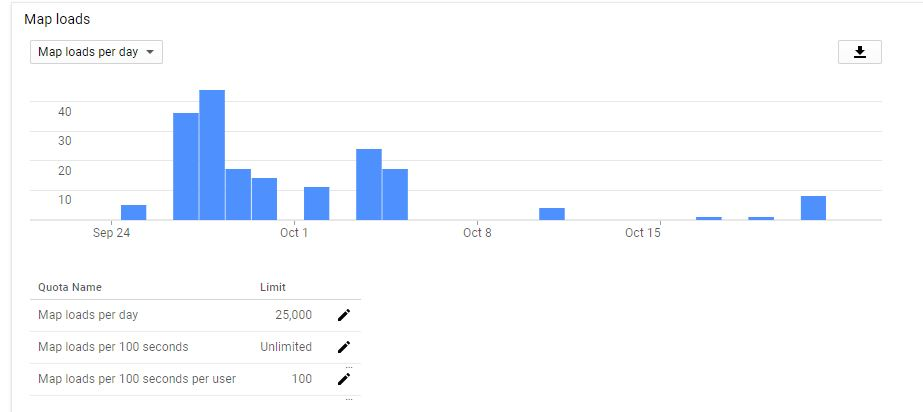
\includegraphics[scale=0.5]{kepek/google_maps_api_1.jpg}
\caption{Adminisztrációs felület}
\label{fig:google_maps_api_1}
\end{figure}

A fent hivatkozott honlapon a kérések monitorozására is lehetőségünk van. Ugyanezen a felületen beállíthatjuk a napi, a 100 másodpercenkénti és a 100 másodperc / felhasználó kérések limitjét (\ref{fig:google_maps_api_2}. ábra).

\begin{figure}[h!]
\centering
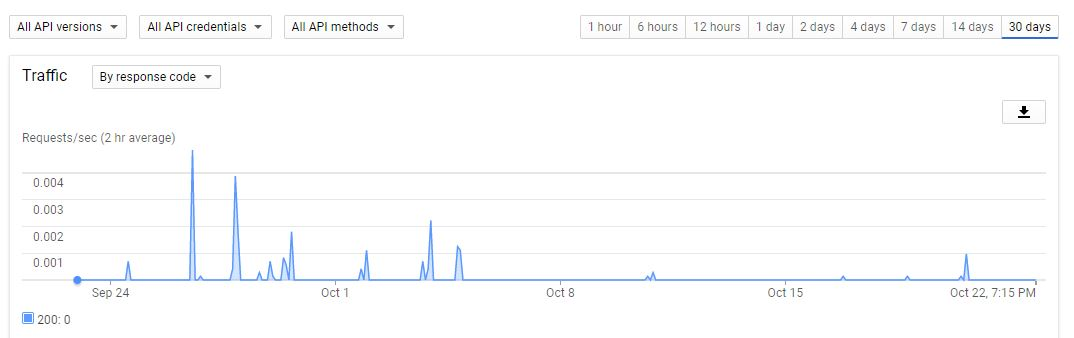
\includegraphics[scale=0.5]{kepek/google_maps_api_2.jpg}
\caption{Hálózati forgalom megjelenítése}
\label{fig:google_maps_api_2}
\end{figure}

Ha beszereztük a szükséges API key-t, akkor azt az oldalunkra be kell linkelni a következő módon:

\begin{verbatim}
<script src="https://maps.googleapis.com/maps/api/js?
key=IDE_KELL_A_KEY-T_BEMASOLNI&callback=drawMap"></script>
\end{verbatim}

A HTML-oldalon elhelyeztem egy \texttt{div}-et, ami a térképet tartalmazza, \texttt{id}-nak \texttt{map}-ot állítottam be. Létrehoztam egy scriptet, ami a \texttt{drawMap} függvényt tartalmazza, ez végzi a térkép manipulálását. A továbbiakban ennek a függvénynek néhány érdekesebb részét ismertetem.

A járatok útvonalai az adatbázisban tárolva vannak. Az adott járathoz tartozó GPS-koordinátákat lekérdezi a függvény a szervertől. Majd egy \texttt{for} cikluson belül ezekből úgynevezett \texttt{LatLng} objektumokat hoz létre a függvény, amit eltárol egy tömbben:

\begin{cpp}
var latlng = new google.maps.LatLng(
    value["shape_pt_lat"],
    value["shape_pt_lon"]
);
shapePoints.push(latlng);
\end{cpp}

Az első paraméter a szélességi, a második a hosszúsági koordináta. Még egy fontos dolog történik a \texttt{for} cikluson belül, egy \texttt{LatLngBounds} objektumot használok a térkép pozícionálásához.

\begin{cpp}
var bounds = new google.maps.LatLngBounds();
\end{cpp}

Ez \texttt{LatLng} objektumok által meghatározott téglalapot reprezentál. A \texttt{LatLngBounds} objektum \texttt{extend} metódusa hívódik meg a cikluson belül, paraméterként átadva az adott iterációban lévő \texttt{LatLng} objektumot, ezáltal a befoglaló téglalapban benne lesz az adott iteráció pontja is:

\begin{cpp}
bounds.extend(latlng);
\end{cpp}

A \texttt{for} ciklus lefutása után a \texttt{bounds} objektum az adott járat összes pontját tartalmazó minimális területű téglalapot fogja tartalmazni.
Hogy a pontokból útvonal legyen, ahhoz egy \texttt{Polyline} objektumot hoz létre a függvény, megadva a tömböt \texttt{path} property-ként. Egyéb beállítási lehetőségeink is vannak, én a vonal színét, átlátszóságát és vastagságát állítottam át, ezt mutatja a következő kódrészlet:

\begin{cpp}
var tripPath = new google.maps.Polyline({
                        path: shapePoints,
                        strokeColor: "#2cc124",
                        strokeOpacity: 0.8,
                        strokeWeight: 4
});
\end{cpp}

Miután ez az objektum is rendelkezésre áll, az útvonalat hozzárendeli a függvény a térképhez, valamint a térképet a befoglaló téglalapra pozícionálja:

\begin{cpp}
tripPath.setMap(map);
map.fitBounds(bounds);
\end{cpp}

A megállók megjelenítése \texttt{markerekkel} történik, megkülönböztetve a végállomásokat és a köztes megállókat. A végállomások tömött zöld körökkel, a köztes megállók zöld szegélyű, fehér kitöltésű körökkel vannak reprezentálva. Az útvonalhoz hasonlóan ebben az esetben is a szervertől lekérdezi a függvény a megállók koordinátáit. Ezt követően szintén egy \texttt{for} cikluson belül ezeken végigiterál, és iterációnként létrehoz egy-egy \texttt{LatLng} objektumot, illetve \texttt{markert}. A \texttt{marker} létrehozását láthatjuk a következő kódrészletben:

\begin{cpp}
var marker = new google.maps.Marker({
    position: latlng,
    icon: {
        path: google.maps.SymbolPath.CIRCLE,
        strokeColor: '#2cc124',
        fillColor: '#FFF',
        fillOpacity: 1,
        scale: 7
    },
    map: map,
    title: value["stop_name"]
});
\end{cpp}

Beállításra kerül a \texttt{marker} pozíciója a létrehozott \texttt{LatLng} objektumból. Az alapértelmezett ikon helyett az \texttt{icon} property megadásával használható más. Mint említettem, én köröket használok, megadva a szegély színét, a kitöltési színt, az átlátszóságot és az ikon nagyságát. A \texttt{markert} hozzá kell rendelni a térkép objektumhoz a \texttt{map} property megadásával. Végül én a \texttt{title} property-t is beállítom, a megálló nevét értékül adva neki. Ezáltal, ha rávisszük a kurzort az ikonra, akkor megjelenik a megálló neve. Ezenkívül \texttt{InfoWindow} ablakokat is használok, ezek akkor jönnek elő, ha egy \texttt{markerre} rákattintunk. Az adott megálló és a járat végállomásának a megállóját tartalmazza. Mindez jól látható \aref{fig:terkep}. ábrán.

\begin{figure}[h!]
\centering
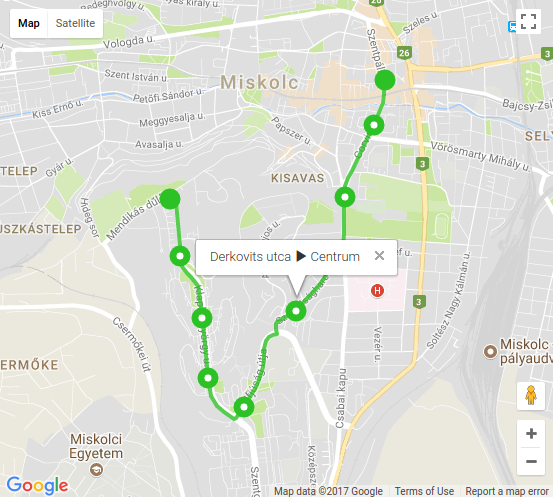
\includegraphics[scale=0.7]{kepek/terkep.png}
\caption{InfoWindow megjelenítése a Google-térképen}
\label{fig:terkep}
\end{figure}

\Chapter{Útvonalkeresés}

\Section{Gráfok ábrázolása}

Az útvonalkereséshez az adatokat gráfokkal kell ábrázolni. A gráfok ábrázolására két adatszerkezet terjedt el. A szomszédsági mátrix, amely tisztán aritmetikai ábrázolású, valamint a szomszédsági lista, amely aritmetikai és láncolt listás ábrázolású \cite{grafabrazolas}.

\SubSection{Szomszédsági mátrix}

Legyen $G = (V,E)$ véges gráf, és $n$ a csúcsok száma. A gráfot $n \times n$-es mátrixszal reprezentáljuk, az oszlopokat és sorokat a csúcsokkal indexeljük (általában $1, \ldots, n$). Egy mező értéke 1, ha a hozzá tartozó oszlop által meghatározott csúcs szomszédja a sor által meghatározott csúcsnak, különben 0, vagyis
$$
C_{i, j} = \begin{cases}
    1, & \text{ha } (i, j) \in E, \\
    0, & \text{ha } (i, j) \notin E. \\
\end{cases}
$$

Az ábrázolásra használt mátrixot \textit{szomszédsági mátrix}nak nevezzük (másnéven \textit{adjacencia} vagy \textit{csúcsmátrix}). Irányítatlan gráf esetén a mátrix szemmetrikus.

% TODO: Ezt majd valamilyen grafikus formában érdemes lehet átszerkeszteni!

\begin{figure}[htb]
\centering
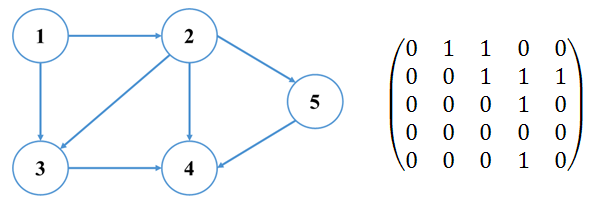
\includegraphics[scale=0.5]{kepek/szomszedsagi_graf_matrix.png}
\caption{Egy irányított gráf és szomszédsági mátrixa.}
\label{fig:szomszedsagi_graf_matrix}
\end{figure}

Súlyozott gráf esetén a súlyok tárolása is a mátrixban történik. Ahol az előző megoldásban 1-es található, tehát létezik az adott él, oda az él költsége kerül.

Az ábrázolás helyfoglalása a mátrix méretének négyzetével, vagyis $n^2$-tel arányos, független az élek számától

\SubSection{Szomszédsági lista}

Ennél a módszernél a gráf minden csomópontjához egy listát rendelünk, amik az adott csúcsból kimenő éleket tartalmazzák.

Legyen $G = (V, E)$ véges gráf, és $n$ a csúcsok száma. Felveszünk egy $Adj[1 \ldots n]$ tömböt, amely mutatókat tartalmaz. A tömb indexelése a csúcsokkal történik. A mutatók az éllistákra (szomszédsági listákra) mutatnak.

Irányított gráf esetén az éleket az éllisták listaelemei reprezentálják. A listaelem tárolása abban a listában történik, amelyik csúcsból az él kiindul. A listaelemben a célcsúcs indexét tároljuk. Az $(i, j) \in E$ él az i-edik listában egy listaelem, melyben j, mint az él célcsúcsa, el van tárolva.

\begin{figure}[htb]
\centering
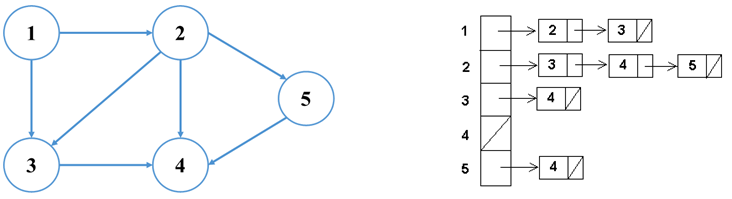
\includegraphics[scale=0.5]{kepek/ellista_iranyitott.png}
\caption{Irányított gráf éllistás ábrázolása.}
\label{fig:ellista_iranyitott}
\end{figure}

Irányítatlan gráf esetében egy élnek két listaelemet is megfeleltetünk. Élsúlyozott gráf esetén, az él súlyát is a listaelemben fogjuk tárolni.

Az ilyen típusú ábrázolás helyfoglalása irányítatlan gráfok esetében a csúcsok számával ($Adj$ tömb) és az élek számával (az éllista elemeinek a számával) arányos, ami összesen $(n + e)$. Irányított gráfoknál az élszám duplájával kell számolni, azaz $(n + 2e)$-vel arányos a helyfoglalás.

\Section{Útvonalkeresés algoritmusa}

Útvonalkeresés során a két pont közötti legrövidebb út megtalálása a cél. A legrövidebb út definíciója \cite{legrovidebbut}:

% TODO: Meg kell nézni, hogy a definíció vége stimmel-e!

,,Legrövidebb út alatt a gráfelméletben egy minimális hosszúságú utat értünk egy gráf két különböző $u$ és $v$ csúcsa között. Amennyiben a gráfunk éleihez nem tartoznak súlyok, akkor ez egyet jelent egy olyan úttal $u$ és $v$ csúcs között, amelyben a legkevesebb él szerepel. Ha vannak súlyok a gráf élein, akkor pedig olyan útról beszélünk, amelynek élein szereplő súlyok összege minimális. Vagyis ha adott egy $G = (V, E)$ gráf, a $k(f), f \in E$ élsúlyokkal, akkor $d(u, v) = \min \Sigma f \in P k(f)$, ahol $P$ út $u$ és $v$ között.''

Algoritmusok
A számos útvonalkereső algoritmus közül kettőt szeretnék részletesebben bemutatni, a Dijkstra-, illetve a Floyd-Warshall-algoritmust.

\SubSection{Dijkstra-algoritmus}

Az algoritmust Edsger Wybe Dijkstra, holland matematikus és informatikus fejlesztette ki 1956-ban. Az algoritmussal a legrövidebb utakat lehet megkeresni egy adott csúcspontból indulva irányított vagy irányítatlan gráfokban egyaránt.

Az algoritmus bemenete egy súlyozott $G$ gráf és a gráf egy $s$ csúcsa. Az út kiinduló pontja az $s$ csúcs. $V$ jelölje a $G$ gráf csúcsainak halmazát, legyen $(u, v)$ a $G$ gráf $u$-t $v$-vel összekötő éle, $u$ és $v$ a gráf csúcsai. $E$ jelölje a $G$ gráf éleinek a halmazát. A $w: E \rightarrow [0, \infty]$ súlyfüggvény az élekhez rendelt súlyokat adja meg, $w(u, v)$ az $(u, v)$ él súlya. Az út költsége két csúcs közt az úton lévő élek összköltsége. Az algoritmus megkeresi a legkisebb költségű $s$-ből $t$-be vezető utat. Ezenkívül arra is alkalmas, hogy adott pontból indulva a gráf minden másik pontjába vezető legrövidebb utat megkeresse.

Az algoritmus működése:

A $G$ gráf minden $v$ csúcsára nyilvántartja az $s$ és $v$ közötti, a futás során addigi legrövidebbnek megtalált út költségét. Induláskor az $s$ csúcsra ez az érték $0$ ($d[s] = 0$), a gráf összes többi csúcsára pedig végtelen ($d[v] = \infty$) minden $v$-re, kivéve $s$). Ennek az az alapja, hogy kezdetben egy utat sem ismerünk, ami az s csúcsból a többibe vezetne. Az algoritmus lefutása után $d[v]$ az $s$-ből $v$-be vezető legrövidebb út költségét tartalmazza, amennyiben létezik út a két csúcs között. Ha nem létezik, akkor $d[v]$ értéke végtelen marad.

Az algoritmus az $S$ és $Q$ halmazokat használja, amelyekben csúcsokat tárol. Az $S$ halmaz a $G$ gráf azon csúcsait tartalmazza, amelyekre $d[v]$ már az odavezető legrövidebb út költségét tartalmazza. A $Q$ halmazban a gráf többi csúcsa található. Kezdetben az $S$ halmaz üres, majd minden egyes iterációval egy csúcs a $Q$ halmazból az $S$ halmazba kerül. Azt a csúcsot választja ki az algoritmus, amelyiknek a legalacsonyabb a $d[u]$ értéke. Amikor az $u$ csúcs a $Q$ halmazból az $S$-be helyeződik, az algoritmus $u$ összes $v$ szomszédjára megvizsgálja, hogy az addig ismert legrövidebb utak tovább rövidíthetőek-e oly módon, hogy a kezdőpontból az $u$-ig vezető legrövidebb úthoz hozzáadjuk az $(u, v)$ él költségét. Ha az eddig ismert legrövidebb útnál kisebb költséget kapunk, akkor $d[v]$ értéke ez az új, kisebb érték lesz.

Az algoritmus pszeudokódja:

\begin{verbatim}
1  function Dijkstra(Graph, s):
 2     for each vertex v in Graph:     
 3         dist[v] := infinity         
 4         previous[v] := undefined
 5     dist[s] := 0                    
 6     Q := copy(Graph)                
 7     while Q is not empty:
 8         u := extract_min(Q)        
 9         for each neighbor v of u:
10             alt = dist[u] + length(u, v)
11             if alt < dist[v]       
12                 dist[v] := alt      
13                 previous[v] := u
\end{verbatim}

Amennyiben csak az $s$-ből $t$-be vezető legrövidebb útra van szükségünk, akkor a keresést a 9. sorban befejezhetjük, ha $u = t$ teljesül. A legrövidebb út meghatározása:

\begin{verbatim}
1 S := empty sequence
2 u := t
3 while defined previous[u]
4     insert u at the beginning of S
5     u := previous[u]
\end{verbatim}

Ekkor $S$ az $s$ csúcsból a $t$-be vezető legrövidebb utak egyikének csúcsait tartalmazó lista, vagy pedig üres, ha nem létezik ilyen út.

Az algoritmus működését szemlélteti az alábbi egyszerű példa.

\begin{figure}[htb]
\centering
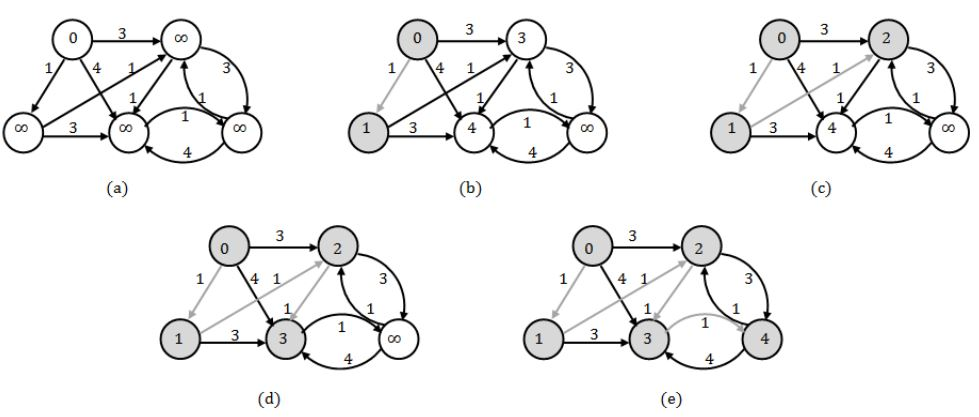
\includegraphics[scale=0.5]{kepek/dijkstra.jpg}
\caption{}
\label{fig:dijkstra}
\end{figure}

\SubSection{Floyd-Warshall-algoritmus}

Két külön algoritmusról van szó, Warshall algoritmusa idősebb a Floyd-algoritmusnál, de a módszerük megegyezik \cite{floyd-warshall}. A szakirodalomban gyakran egyként kezelik a két algoritmust a hasonlóságuk miatt, és Floyd-Warshall néven hivatkoznak rá.
A különbség az algoritmusok közt, hogy a Warshall-algoritmus csak arra ad megoldást, hogy mely pontok közt található irányított út, nem adja meg azok hosszát.

A Floyd-Warshall-algoritmus pszeudokódja:

% TODO: A pszeudó-kódot érdemes lehet kicsit átfogalmazni inkább!

\begin{verbatim}
1 let dist be a |V| x |V| array of minimum distances initialized to oo (infinity)
2 for each vertex v
3    dist[v][v] <- 0
4 for each edge (u,v)
5    dist[u][v] <- w(u,v)  // the weight of the edge (u,v)
6 for k from 1 to |V|
7    for i from 1 to |V|
8       for j from 1 to |V|
9          if dist[i][j] > dist[i][k] + dist[k][j] 
10             dist[i][j] <- dist[i][k] + dist[k][j]
11         end if
\end{verbatim}

Az algoritmus lépésszáma a három egymásba ágyazott for ciklus miatt n3-bel arányos. Ez nagyságrendben ugyanannyi, mint a Dijkstra-algoritmus mátrixos változata, de a Floyd-módszer 50%-kal gyorsabb. Amennyiben a gráf éleinek száma kisebb, mint 2 n , és az élsúlyok nemnegatívak, akkor viszont a Dijkstra-algoritmus éllistás változatát érdemesebb használni.

\SubSection{Útvonaltervezés implementálása}

Az elméleti áttekintés után térjünk rá az útvonaltervezés implementációjára. Mivel ez egy viszonylag komplex probléma, így több iterációban történt az implementálás. Első körben csak a natív, irányítatlan gráfot hoztam létre a GTFS-adatokból, és az ebben való keresésre implementáltam a Dijkstra-algoritmust. Miután ezt sikerült megvalósítani, fokozatosan építettem be a további feltételeket, megszorításokat a gráfgeneráló és az útvonalkereső algoritmusba.

Első körben a gráfot dictionary-k dictonary-eként hoztam létre. A külső dictionary-ben a kulcsok az egyes megállók nevei, az érték pedig egy másik dictionary. A belső dictionary-ben a kulcsok szintén megállónevek. Jelentésük, hogy a külső megállóból ebbe a megállóba közvetlenül el lehet jutni. Ebben a fázisban azt még nem tartalmazta a gráf, hogy ezt melyik viszonylaton (viszonylatokon) keresztül lehet megtenni. A belső dictionary-ben az értékek a költséget jelentik, hány másodperc alatt lehet eljutni egyik megállóból a másikba. Ezáltal egy súlyozott, irányított gráf épült fel az adatokból, a súlyozás a másodpercben kifejezett időköltség a két megálló közt.

Egy részlet az így felépített gráfból:

\begin{verbatim}
{
    'AUCHAN Borsod': {'Szondi György utca': 300.0},
    'AUCHAN-dél (Pesti út)': {
        'Pesti út': 60.0,
        'Sütő János utca': 300.0
    },
    'Aba utca': {
        'Zoltán utca': 60.0,
        'Szent Anna tér': 120.0
    },
    'Alföldi utca': {
        'Orvosi rendelő': 60.0
    },
    'Alsó-Hámor': {
        'Felső-Hámor': 60.0,
        'Csanyik-völgy': 60.0
    },
    'Alsó-Majláth': {
        'Felső-Majláth': 120.0,
        'Diósgyőr városközpont': 120.0,
        'Bölcs utca': 60.0,
        'Móra Ferenc utca': 120.0},
    ...
}
\end{verbatim}

Jól látható, hogy az AUCHAN Borsod megállóból egyedül a Szondi György utca megállóba tudunk eljutni, 300 másodperc alatt. Ezzel szemben például az Alsó-Majláth megállóból indulva eljuthatunk 120 másodperc alatt Felső-Majláth, Diósgyőr városközpont és a Móra Ferenc utca megállókba, 60 másodperc alatt pedig a Bölcs utcába.

Miután a gráfgeneráló algoritmust elkészítettem, a Dijkstra-algoritmus implementálása következett.

A függvény három paramétert vár, a gráfot, valamint kezdő- és végpontot, tehát két megálló nevét. Először egy ellenőrzés történik, hogy a paraméterként megadott megállók szerepelnek-e a gráfban. Ha igen, megkeresi a legrövidebb utat köztük. Két értékkel tér vissza, a path tartalmazza a kiszámolt utat, a cost értéke pedig az út időköltsége lesz.
Egy példa a függvény meghívására:

\begin{verbatim}
path, cost = dijkstra(graph, 'Egyetemváros', 'Selyemrét')
\end{verbatim}

A függvény által kiszámolt út (path tartalma):

\begin{verbatim}
[
    'Egyetemváros',
    'Olajkutató',
    'Egyetemi Kollégium',
    'Csermőkei út',
    'Szentgyörgy út',
    'Vasúti felüljáró',
    'Tapolcai elágazás',
    'Petneházy utca',
    'Lévay József utca',
    'Vízügyi Igazgatóság',
    'Selyemrét'
]
\end{verbatim}

Az eredményt egy listában adja vissza, amely a megállók neveit tartalmazza. A cost értéke pedig 780 ebben a példában.

Miután ezzel elkészültem, a gráfot kibővítettem, hiszen nem elegendő csak annyit tudni, hogy egy megállóból mely másikakba vezet út. Azt is el kell tárolni, hogy ez a kapcsolat melyik viszonylaton érhető el. Olyan is előfordulhat, hogy A-ból B-be több viszonylaton is el lehet jutni, az optimális útvonal megtervezéséhez ezt is figyelembe kell venni, nem elég csupán egy viszonylatot eltárolni.
Mindezek figyelembevételével átalakítottam a gráf struktúráját. Továbbra is egy dictionary-ről van szó, ahol a kulcsok a megállók nevei, az értékek azonban listák. A listákban dictionary-k vannak, mindegyik dictionary-ben pedig három kulcs-érték pár. A name-hez tartozó érték a megálló neve, a cost a költség, a route pedig a viszonylatot azonosítja.
Részlet a kibővített gráfról:

\begin{verbatim}
{'AUCHAN Borsod': [{
    'name': 'Szondi György utca',
    'cost': 300.0,
    'route': 'AU1'
}],
'AUCHAN-dél (Pesti út)': [{
    'name': 'Pesti út',
    'cost': 60.0,
    'route': '44'
}, {
    'name': 'Sütő János utca',
    'cost': 300.0,
    'route': 'AU2'
}],
'Aba utca': [{
    'name': 'Zoltán utca',
    'cost': 60.0,
    'route': '1'
}, {
    'name': 'Szent Anna tér',
    'cost': 120.0,
    'route': '1'
}, {
    'name': 'Zoltán utca',
    'cost': 60.0,
    'route': '1É'
}, {
    'name': 'Szent Anna tér',
    'cost': 120.0,
    'route': '1É'
}, {
    'name': 'Zoltán utca',
    'cost': 60.0,
    'route': '54'
}, {
    'name': 'Szent Anna tér',
    'cost': 120.0,
    'route': '54'
}], ...
}
\end{verbatim}

Az Aba utca megállóhoz tartozó bejegyzést, ha jobban szemügyre vesszük, könnyen megérthetjük, hogy milyen változás történt. Míg az előző változatban annyi információt tároltunk csak el, hogy a Zoltán utca és a Szent Anna tér megállókba lehet innen eljutni 60 és 120 másodperc alatt ('Aba utca': {'Zoltán utca': 60.0, 'Szent Anna tér': 120.0}), addig a kibővített gráf sokkal több információt tartalmaz. Láthatjuk, hogy mindkét irányba három viszonylaton is (1, 1É, 54) eljuthatunk. Így a gráf mérete a többszörösére növekedett, azonban ez a változtatás elengedhetetlen volt, hiszen az útvonaltervezésnek csak úgy van értelme, ha a viszonylatokat is figyelembe vesszük.

Ezután természetesen az útvonaltervező algoritmust és át kellett írni, hogy kezelni tudja az átalakított struktúrájú gráfot.

Az átalakítás után, az előző példánál maradva, ha kipróbáljuk az Egyetemváros és a Selyemrét megállókkal az algoritmust, akkor a path eredménye a következő lesz:

\begin{verbatim}
[{
    'name': 'Egyetemváros', 'route': '12'
}, {
    'name': 'Olajkutató', 'route': '12'
}, {
    'name': 'Egyetemi Kollégium', 'route': '12'
}, {
    'name': 'Csermőkei út', 'route': '20'
}, {
    'name': 'Szentgyörgy út', 'route': '12'
}, {
    'name': 'Vasúti felüljáró', 'route': '12'
}, {
    'name': 'Tapolcai elágazás', 'route': '30'
}, {
    'name': 'Petneházy utca', 'route': '32'
}, {
    'name': 'Lévay József utca', 'route': '4'
}, {
    'name': 'Vízügyi Igazgatóság', 'route': '4'
}, {
    'name': 'Selyemrét', 'route': None
}]
\end{verbatim}

Az eredményt szintén egy listában adja vissza, azonban a listában most már nem csak pusztán a megállók nevei vannak, hanem dictionary-kben név és viszonylat kulcs-érték párok. A megváltozott felépítésű gráfot már tudja kezelni az algoritmus, azonban az átszállásokra nézve még nem ad optimális eredményt.


\Chapter{További funkciók}

Külön fejezetekbe kerülhetnek a további funkciók, vagy komplikáltabb megoldások. Csak ötlet szintjén:
- Következő ajánlott útvonal számítása az aktuális idő, kiindulópont és a célállomás ismeretében. (Az útvonalkereső is gyakorlatilag ezt csinálja, itt annyi a különbség, hogy kvázi kiírja a felhasználónak, hogy merre érdemes indulnia, és vált, ha közben megváltozik a javaslat az eltelt idő miatt.)
- Menetrend mentése valamilyen nyomtatható formában.
- Minimalizálás az átszállások számára vonatkozóan.
- Kieső járattal kapcsolatos számítások.
- Várakozási idők minimalizálása, vagy limit az átszállásra vonatkozóan (például több legyen, mint 3 perc, hogy biztos legyen idő átszállni).
\Chapter{Tesztelés}

Az elkészített alkalmazást kipróbáltam több különböző közlekedési társaság GTFS-adatbázisával is. Ehhez az adatokat a \url{https://transitfeeds.com} oldalról szereztem be. Az oldal nyilvános GTFS-adatbázisok archívuma, elsősorban szoftverfejlesztők számára, a világ minden tájáról összegyűjtve. Jelenleg több mint 500 különböző város menetrendjének az archívuma található az oldalon. Ezek közül választottam ki hatot, amelyekkel teszteltem az alkalmazásomat. Négy magyarországi (Budapest, Miskolc, Szeged, Pécs) és két külföldi (Bécs, Firenze) várost választottam.

Megvizsgáltam, hogy a nyers adatokból mennyi idő alatt jön létre az adatbázis a GTFSDB \texttt{database\_load} függvényével. Az eredményeket összesíti \aref{tab:gtfs}. táblázat.

\begin{table}
\centering
\begin{tabular}{|l|r|r|r|r|}
\hline
Menetrend & ZIP mérete (MB) & \texttt{trips} bejegyzések száma & \texttt{stop\_times} bejegyzések száma & Betöltési idő (másodperc) \\
\hline
Bécs & 14,6 & 120 181 & 2 169 529 & 1 395 \\
\hline
Budapest & 39,3 & 227 900 & 4 518 698 & 2 945 \\
\hline
Firenze & 10 & 40 683 & 1 017 698 & 836 \\
\hline
Miskolc & 1,2 & 9 641 & 148 785 & 97 \\
\hline
Szeged & 1,9 & 17 162 & 302 816 & 191 \\
\hline
Pécs & 1,5 & 5 563 & 111 192 & 71 \\
\hline
\end{tabular}
\caption{GTFS adatbázisok mennyiségi jellemzői és betöltési ideje}
\label{tab:gtfs}
\end{table}

A táblázatban látható a letöltött adatfájl mérete, a betöltési idő másodpercben, illetve hogy a \texttt{trips} és a \texttt{stop\_times} táblák hány darab rekordból állnak. Azért ezt a kettőt emeltem ki, mert legnagyobb részt ezek határozzák meg, hogy mennyi lesz a betöltési idő. Kisebb városok esetén, ahol néhány százezer rekordról van szó, viszonylag hamar, 1-3 perc alatt fel lehet tölteni az adatbázist. Nagyobb, több millió rekordból álló adathalmaz esetén ez már több 10 percig is eltart. Általában egy GTFS feed egy hónapra előre tartalmazza a menetrendet, ezért ezt a műveletet ritkán kell elvégezni. Mivel általában nem változik hónapról hónapra drasztikusan a menetrend, ezért elegendő lehet csak a \texttt{calendar} és a \texttt{calendar\_dates} táblák aktualizálása a következő havi dátumokkal, valamint az esetleges megváltozott menetrendű járatok frissítése, az adatbázis legnagyobb részét elegendő egyszer feltölteni, és az utána hosszú hónapokig aktuális marad.

Készítettem egy statisztikát, hogy a \texttt{generate\_graph} függvény mennyi idő alatt fut le, vagyis az adott hálózat megállóiból mennyi idő alatt építi fel az útvonalkereséshez a gráfot. Ugyanazokat az adatbázisokat használtam, amiket az előző teszthez összegyűjtöttem. Ezt foglalja össze \aref{tab:runtime}. táblázat.

\begin{table}
\centering
\begin{tabular}{|l|r|r|}
\hline
Menetrend & Megállók száma & \texttt{generate\_graph} futási ideje (másodperc) \\
\hline
Bécs & 4 357 & 17,3 \\
\hline
Budapest & 7 391 & 28,7 \\
\hline
Firenze & 2 307 & 10,3 \\
\hline
Miskolc & 561 & 3,1 \\
\hline
Szeged & 574 & 2,9 \\
\hline
Pécs & 541 & 2,6 \\
\hline
\end{tabular}
\caption{Gráf generálásának futási ideje a futási idő függvényében}
\label{tab:runtime}
\end{table}

Hasonlóan az adatbázisok betöltési idejéhez, a gráf felépítésének ideje is az adatbázis méretével arányos. Ebben az esetben a megállók száma a mérvadó, hiszen a készítendő gráfnak ugyanannyi csomópontja lesz, illetve az élek számával is arányos. A megfelelő felhasználói élmény biztosítása érdekében a gráfot egyszer kell felépíteni, és az eredményt gyorsítótárban kell tárolni.

\Chapter{Összegzés}

%* Ezt elég lesz majd csak a végén megcsinálni.
%* Ebben már csak át kell majd tekinteni az elkészült dolgokat.
%* 1-2 oldalnál (a bevezetéshez hasonlóan) ennek sem kell hosszabbnak lennie.

A szakdolgozatom célja egy olyan webalkalmazás készítése volt, melyben a menetrendadatok a nemzetközi szabvánnyá vált GTFS-formátumban vannak tárolva, a menetrend böngészése könnyen átlátható formában valósul meg a felhasználók számára, amit útvonaltervező funkció is segít. Az alkalmazás elkészítéséhez kliensoldalon AngularJS-t, szerveroldalon pedig Python / Flask keretrendszert használtam. Sikerült egy olyan alkalmazást készíteni, amely a GTFSDB library segítségével bármelyik GTFS-t használó közlekedési vállalat menetrendi adataival kompatibilis.

Az elkészített alkalmazás már a jelenlegi állapotában is használható, a megvalósítani kívánt funkciók egytől egyig működőképesek. Vannak azonban ötleteim a későbbi továbbfejlesztési lehetőségekre, néhányat ismertetnék ezek közül. Véleményem szerint leginkább az útvonaltervező funkciót lehetne tovább finomítani, kibővíteni még több lehetőséggel. Ilyen lehetne például a következő ajánlott útvonal számítása az aktuális idő, kiindulópont és a célállomás ismeretében. Hasznos lehetne az átszállások számát minimalizáló opciót, vagy a várakozási idők minimalizálását implementálni, amit a felhasználó ki tudna választani, hogy milyen szempont szerinti optimális útvonaltervet szeretne. Szóba jöhetne egy limit az átszállásra vonatkozóan, például több legyen, mint három perc, hogy biztosan elegendő idő legyen az átszállásra. A menetrend böngészése kapcsán továbbfejlesztési lehetőségként az egyes viszonylatok menetrendjének a nyomtatható formában történő mentésének a támogatása is egy hasznos ötletnek tűnik. Nagyon érdekes lehet még az ismert megállók, és az azokat összekötő útvonalak esetében kiszámolni egy lehetséges – valamilyen szempontból optimális – menetrendet, ami tehát a keresési problémának a megfordítása lenne.

\Chapter{Summary}

The goal of my thesis work was to create a web application which stores the schedule information in GTFS format. This format has become an international standard. The browsing of the schedule information is easy via the web interface. It also provides functions for trip planning. I used AngularJS on the client side and Python / Flask framework on the server side. I developed an application with the GTFSDB library, which is compatible with the timetable of any transit agency using GTFS.

The created application is ready to use in its current state. Each of the planned functions have been implemented. However, I have some ideas for further development. I would like to mention some of these. In my opinion, the trip planning function could be refined by adding more options. For example, it can calculate the following recommended route based on the current time, a starting point, and a destination. It could be useful to minimize the number of transfers or waiting times. The user would be able to choose the optimization criteria for finding the appropriate route. There could be a limit on the transfer, for example more than three minutes is enough time to transfer. As a further option for browsing the timetable, it could be implemented a function for export the timetable to a printable format. It may be very interesting to calculate an optimum timetable from some points of view based on known stops and routes connecting them. In fact, it is the inverse of the search problem.


\begin{thebibliography}{x}
\addcontentsline{toc}{chapter}{\bibname}

\bibitem{python} https://hu.wikipedia.org/wiki/Python\_(programoz%C3%A1si\_nyelv) 

\bibitem{flask} 

\bibitem{sqlalchemy} https://hu.wikipedia.org/wiki/SQLAlchemy

\bibitem{html} https://hu.wikipedia.org/wiki/HTML

\bibitem{javascrip} https://developer.mozilla.org/hu/docs/Web/JavaScript

\bibitem{angularjs} http://nyelvek.inf.elte.hu/leirasok/JavaScript/index.php?chapter=27

\bibitem{css} https://hu.wikipedia.org/wiki/Cascading\_Style\_Sheets

\bibitem{bootstrap} http://nora707.tryfruit.com/2016/10/25/bootstrap/

\bibitem{git} https://into.hu/hirek/csapatmunka-git-el-1-resz-mi-is-az-a-git

\bibitem{github}

\bibitem{gtfs}
https://developers.google.com/transit/gtfs/

\bibitem{gtfsspec}
https://en.wikipedia.org/wiki/General\_Transit\_Feed\_Specification

\bibitem{grafabrazolas}
http://tamop412.elte.hu/tananyagok/algoritmusok/lecke23\_lap1.html

\bibitem{legrovidebbut}
https://web.cs.elte.hu/blobs/diplomamunkak/bsc\_matelem/2009/podobni\_katalin.pdf

\bibitem{dijkstra}
https://hu.wikipedia.org/wiki/Dijkstra-algoritmus

\bibitem{floyd-warshall}
https://web.cs.elte.hu/blobs/diplomamunkak/bsc\_matelem/2009/podobni\_katalin.pdf

\end{thebibliography}


% \Chapter{CD-melléklet tartalma}

Dolgozatomhoz egy darab CD-melléklet tartozik, melynek tartalma a következő:

\bigskip

\noindent \texttt{Dolgozat} katalógus:

\begin{itemize}
\item \texttt{GTFS-alapu\_menetrendnyilvantarto-rendszer.pdf}: \\ A dolgozatot tartalmazó fájl, PDF-formátumban.
\item \texttt{kiiras.pdf}: A feladatkiírást tartalmazó fájl, PDF-formátumban.
\item \texttt{osszefoglalas.pdf}: Magyar nyelvű összefoglaló, PDF-formátumban.
\item \texttt{osszefoglalas.tex}: Magyar nyelvű összefoglaló, \LaTeX-formátumban.
\item \texttt{summary.pdf}: Angol nyelvű összefoglaló, PDF-formátumban.
\item \texttt{summary.tex}: Angol nyelvű összefoglaló, \LaTeX-formátumban.
\end{itemize}

\bigskip

\noindent \texttt{LaTeX} katalógus:

A dolgozat \LaTeX-kódját tartalmazza.

\bigskip

\noindent \texttt{Forraskod} katalógus:

Az alkalmazás forráskódját tartalmazza.


\end{document}
